
\subsection{$\PH \to \ZZ \to 2\ell 2\ell '$}

The events are selected by the triggers that require the presence of a
pair of electrons, or a pair of muons, or
an electron and a muon.
%The requirements on the transverse energy (transverse momenta) for
%the first and second lepton are 17 and 8\GeV respectively.
%The trigger efficiency within the acceptance of this analysis is greater than 99\% (96\%, 98\%)
%for a Higgs boson signal 
%with $\mH > 180\GeV$.
The reconstructed electrons or muons from \cPZ\ decays should be isolated and 
originate from the
primary vertex. A detailed description of the analysis can 
be found in~\cite{cmsobsboson,Chatrchyan:2012dg,Chatrchyan:2012hr}.  
%The lepton isolation requirements suppress the Z+jet, Z$b\bar{b}$ and $t\bar{t}$ 
%backgrounds. 
%This is ensured by requiring that the significance of
%the impact parameter to the event vertex, ${\rm SIP_{3D}}$, satisfies
%$| {\rm SIP_{3D}} = \frac{\rm IP}{\sigma_{\rm IP}} | < 4$ for each
%lepton. The ${\rm IP}$ is the lepton impact parameter in three
%dimensions at the point of closest approach with respect to the
%primary interaction vertex, and $\sigma_{\rm IP}$ the associated
%uncertainty.
%These requirements 
%on the significance of the impact parameter to the event vertex
%suppresses posible contribution from the 
%$\cPZ$+jet, $\cPZ b\bar{b}$ and $t\bar{t}$ background processes. 
%%Photons reconstructed within $\vert \eta^{\gamma} \vert < 2.4$ are
%%considered as possible final state radiation (FSR) candidates
%%if they have $p_{\rm T}^\gamma > 2 \GeV $ ($p_{\rm T}^\gamma > 4\GeV $) and are found
%%within a conical distance $ \Delta R < 0.07 $ ($ 0.07 < \Delta R < 0.5 $)
%% from a selected lepton
%%candidate.
%%In the latter case the photons are required to be isolated and
%%satisfy $R_{\rm Iso}^{\gamma} < 1$.
%%The photon isolation observable $R_{\rm
%%Iso}^{\gamma}$ is obtained by summing over the transverse momenta of
%%charged hadrons, other photons and neutral hadrons 
%identified by the
%PF reconstruction 
%%in a cone of size $\Delta R = 0.3$ around the
%%candidate photon direction, correcting for pileup, and dividing by the
%%photon transverse momentum, $p_{\rm T}^\gamma$. 
%The performance of the FSR selection algorithm has been measured using
%MC simulation samples, and the rate was verified with single-\cPZ\
%data events.  
%%The photons within the acceptance for the FSR selection
%%are measured with an efficiency of $\simeq 50\%$ and with a mean
%%purity of $80\%$.  FSR photons are selected in 5\% of single-\cPZ\
%%events with muon pairs, and 0.5\% of single-\cPZ\ events with electron
%%pairs.  A gain of $\simeq 3\%$ (2$\%$, 1$\%$) in efficiency is
%%achieved.
%%When building the \cPZ\ candidates, only the FSR photons associated with the closest
%%lepton and which make the "dressed" lepton-pair mass closer to the nominal
%% \cPZ\  mass are kept, with a maximum mass $m_{\ell\ell\gamma}<100 \GeV$. 

We require a \cPZ\ candidate formed with a pair of leptons of the same 
flavour and  opposite charge ($\ell^+\ell^-$). Electrons (muons) are required to 
have $\pt > 7(5)\GeV$ and $|\eta|<2.5(2.1)$. 
The $\tau_h$ are required to have $\PT > 20 \GeV$ and $|\eta|<2.3$.
The event selection is built to give a mutually exclusive set of signal candidates 
in the  $\PH\rightarrow 2\ell 2\ell$ and $\PH\rightarrow 2\ell2\Pgt$ channels. 
The signal candidates in the $2\ell 2\ell$ analysis are first selected. 

In the $2\ell2\ell$ final state, 
the pair with an invariant mass closest to the nominal \cPZ\  mass is denoted
$m_{\cPZ_1}$ and retained if it satisfies $40 < m_{\cPZ_1} < 120\GeV$.
We then consider all remaining leptons and require a second pair of $\ell^+\ell^-$,
with mass denoted $m_{\cPZ_2}$, to satisfy $12 < m_{\cPZ_2} < 120\GeV$.
If more than one ${\cPZ_2}$ candidate satisfies all criteria, the ambiguity
is resolved by choosing the leptons of highest \PT.
Among the four selected leptons forming $\cPZ_1$ and the $\cPZ_2$,
at least one should have $\PT > 20 \GeV$ and another one 
have $\PT > 10 \GeV$.
These \PT thresholds ensure that the selected events have leptons 
on the high-efficiency plateau of the trigger.
%To further protect against leptons originating from hadron decays in jet fragmentation 
%or from the decay of low-mass hadronic resonances, we require that any 
%opposite-charge pair of leptons chosen among the four selected leptons (irrespective of flavour)
%satisfy $m_{\ell\ell'} > 4\GeV$.

For the search in the $2\ell2\Pgt$ final state, events are required to have one 
$\cPZ_1 \to \ell^+\ell^-$ candidate with one lepton at $\PT > 20 \GeV$ and the other at
$\PT > 10 \GeV$,
and a  $\cPZ_2 \to \Pgt^+\Pgt^-$, with $\Pgt$ decaying into $\Pgm, \Pe$ or $\tauh$.
The leptons from the \Pgt\ leptonic decays are required to have $\PT > 10 \GeV$. 
The invariant mass of the reconstructed $\cPZ_1$ is required to satisfy
$ 60 < m_{\ell\ell} < 120\GeV$, and that of the $\cPZ_2$ to satisfy
$ m_{\Pgt\Pgt} < 90\GeV$, where $m_{\Pgt\Pgt}$ is the invariant mass of the visible 
tau-decay products.

We rely on MC simulation to evaluate the local density ($\Delta N /
\Delta m_{2\ell2\ell'}$) of events expected as a function of 
$m_{2\ell2\ell'}$ from the \cPZ\cPZ\ background.  
%Following the prescription
%used in the previous analysis, 
The cross section for \ZZ\
production at NLO is calculated with
\textsc{mcfm}~\cite{MCFM,Campbell:1999ah,Campbell:2011bn}.
%This includes the dominant process of $\Pq\Paq$ annihilation,  as well as gluon fusion.
The theoretical uncertainties are computed as a function of $m_{2\ell2\ell'}$, 
varying both the QCD renormalisation
and factorization scales and the PDF set, following the PDF4LHC
recommendations~\cite{Botje:2011sn,Alekhin:2011sk,Lai:2010vv,Martin:2009iq,Ball:2011mu}.
The uncertainties for the QCD and PDF scales for each final state are on average 8\%.
The number of predicted $\ZZ \to 2\ell 2\ell'$  events and their uncertainties after the signal
selection are given in Table~\ref{tab:SelectYields}.

To estimate the reducible 
$\ttbar$, $\cPZ$jets, and $\PW\cPZ$+jets
backgrounds, a $\cPZ_1$+X background control region, 
%($\cPZ\bbbar$, $\ttbar$) and instrumental ($\cPZ+\text{light jets}$, $\PW\cPZ+\text{jets}$)
well separated from the signal region, is defined. 
In addition, a sample $\cPZ_1 + \ell_\text{reco}$, with at least one reconstructed lepton object is
defined for the measurement of the lepton misidentification probability --- the probability for a
reconstructed object to pass the isolation and identification requirements.
The contamination from \PW\cPZ\ in these events is suppressed by requiring the imbalance
of the measured energy deposition in the transverse plane to be below $25\GeV$.
%The lepton misidentification probability is compared, and found compatible, with the one
%derived from MC simulation.
The event rates measured in the background control region are extrapolated to the
signal region
and presented in Table~\ref{tab:SelectYields}. The systematic uncertainies of the 
reducible background estimate vary between 30\% and 100\% and are presented in the table 
together with statistical uncertainties squared. 

%For the $4\ell$ background estimate, two different approaches are used. 
%Both start by relaxing the isolation and identification criteria for two additional reconstructed 
%lepton objects.
%A first approach follows from the previous CMS analysis.
%The additional pair of leptons is required to have the same charge (to avoid signal contamination)
%and same flavour ($\Pe^{\pm}\Pe^{\pm}, \Pgm^{\pm}\Pgm^{\pm}$), a reconstructed invariant 
%mass $m_{\cPZ_2} > 12 \GeV$, and $m_{4\ell} > 100\GeV$.
%The expected number of $\cPZ$+X background events in the signal region is obtained by taking
%into account the lepton misidentification probability for each of the two additional leptons.
%The second method uses the control region with two opposite-sign leptons failing the isolation 
%and identification criteria, and using the misidentification probability to extrapolation to the signal region. 
%In addition, a control region with three passing and one failing lepton is also used to 
%account for contributions from backgrounds with three prompt leptons and one misidentified lepton. 
%Comparable background counts in the signal region are found within uncertainties from
%both methods. An envelope comprising these results is used as the final estimate in
%Table~\ref{tab:SelectYields}.

%============
\begin{table}[htbp]
\begin{center}
\caption{
The number of event candidates observed, compared to the mean expected 
background and signal rates for each final state.
For the $\cPZ$+X background, the estimations are based on data.
%The results are given integrated over the full mass measurement range 
%for the Higgs boson search from 100 to 800\GeV.
%and in the low mass range from 100 to 130\GeV.
The uncertainties represent the statistical and systematic uncertainties squared.
}
\label{tab:SelectYields}
\begin{tabular}{l|c|c|c|c|c}
\hline
\textbf{Channel} & $4\Pe$ & $4\Pgm$ & $2\Pe2\Pgm$ & $4\ell$ & $2\ell2\Pgt$  \\
\hline
\cPZ\cPZ\ background &  29.3  $\pm$  3.4 &  49.0  $\pm$  5.1  &  75.5  $\pm$  8.0 &  153.7 $\pm$ 10.1 & 12.1 $\pm$ 1.5 \\ %
\cPZ+X                            &   $3.0 ^{ +  2.7 }_{ -  1.9 }$ &  $2.2 ^{ +  1.6 }_{ -  1.3 }$ &  $5.0 ^{ +  4.0 }_{ -  3.0 }$  & $10.2 ^{ +  5.0 }_{ -  3.8 }$ & 8.9  $\pm$ 2.5  \\ % 
\hline
All backgrounds    &   $32.3 ^{ +  4.4 }_{ -  3.9 }$ &  $51.2 ^{ +  5.3 }_{ -  5.3 }$ &  $80.5 ^{ +  9.0 }_{ -  8.6 }$ &  $163.9 ^{ +  11.3 }_{ -  10.8 }$ & 21.0 $\pm$ 2.9  \\ % 
%~~~($100 < m_{4\ell} < 130\GeV$)   &    X.XX $\pm$ XX  & X.XX $\pm$ XX &   X.XX $\pm$ XX  & --  \\ % 5/fb
\hline
Observed  & 32 & 47  & 93 & 172 & 20 \\ % 5/fb
\hline
$\mH = 200\GeV$ & 8.3  $\pm$  2.0  &  13.3  $\pm$  2.7  &  21.6  $\pm$  4.5 &  43.2  $\pm$ 5.6 &  2.9 $\pm$ 0.7  \\ % 
$\mH = 350\GeV$ & 4.8  $\pm$  1.2  &  7.5  $\pm$  1.6  &  12.7  $\pm$  2.9 &  24.9  $\pm$  3.5 &  3.1 $\pm$ 0.8 \\ % 
$\mH = 500\GeV$ & 1.7  $\pm$  0.8  &  2.6  $\pm$  1.2  &  4.4  $\pm$  2.0 &  8.7  $\pm$  2.4 &   1.4 $\pm$ 0.7 \\ % 
\hline
\end{tabular}
\end{center}
\end{table}

The reconstructed four-lepton invariant-mass distributions for the $2\ell 2\ell$, combining the
$4\Pe$, $4\Pgm$, and  $2\Pe2\Pgm$ channels, are shown in Fig.~\ref{fig:Mass4l-2l2tau}(a) 
and compared with the expectation from SM background processes.
%=============
\begin{figure}[htbp]
\begin{center}
%
%{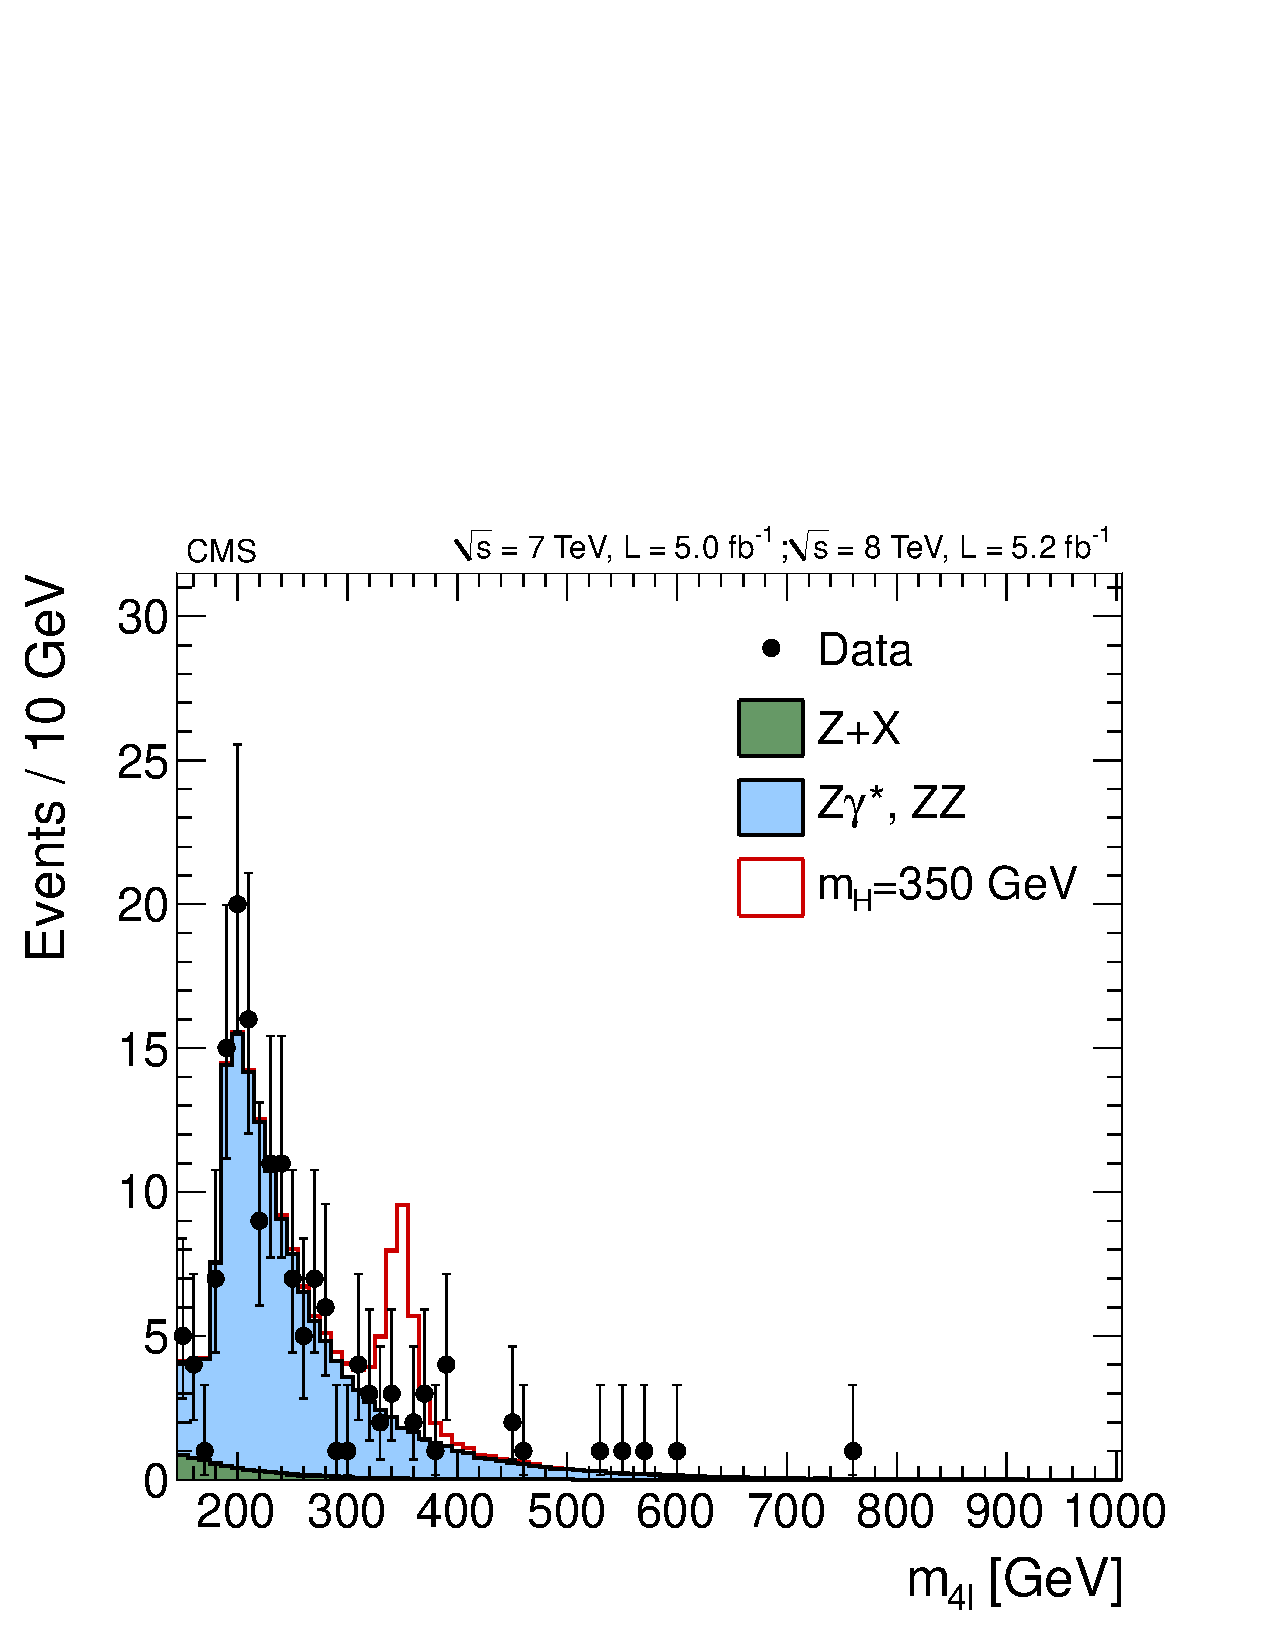
\includegraphics[width=0.44\textwidth]{plots/hzz4lmass.pdf}}
%{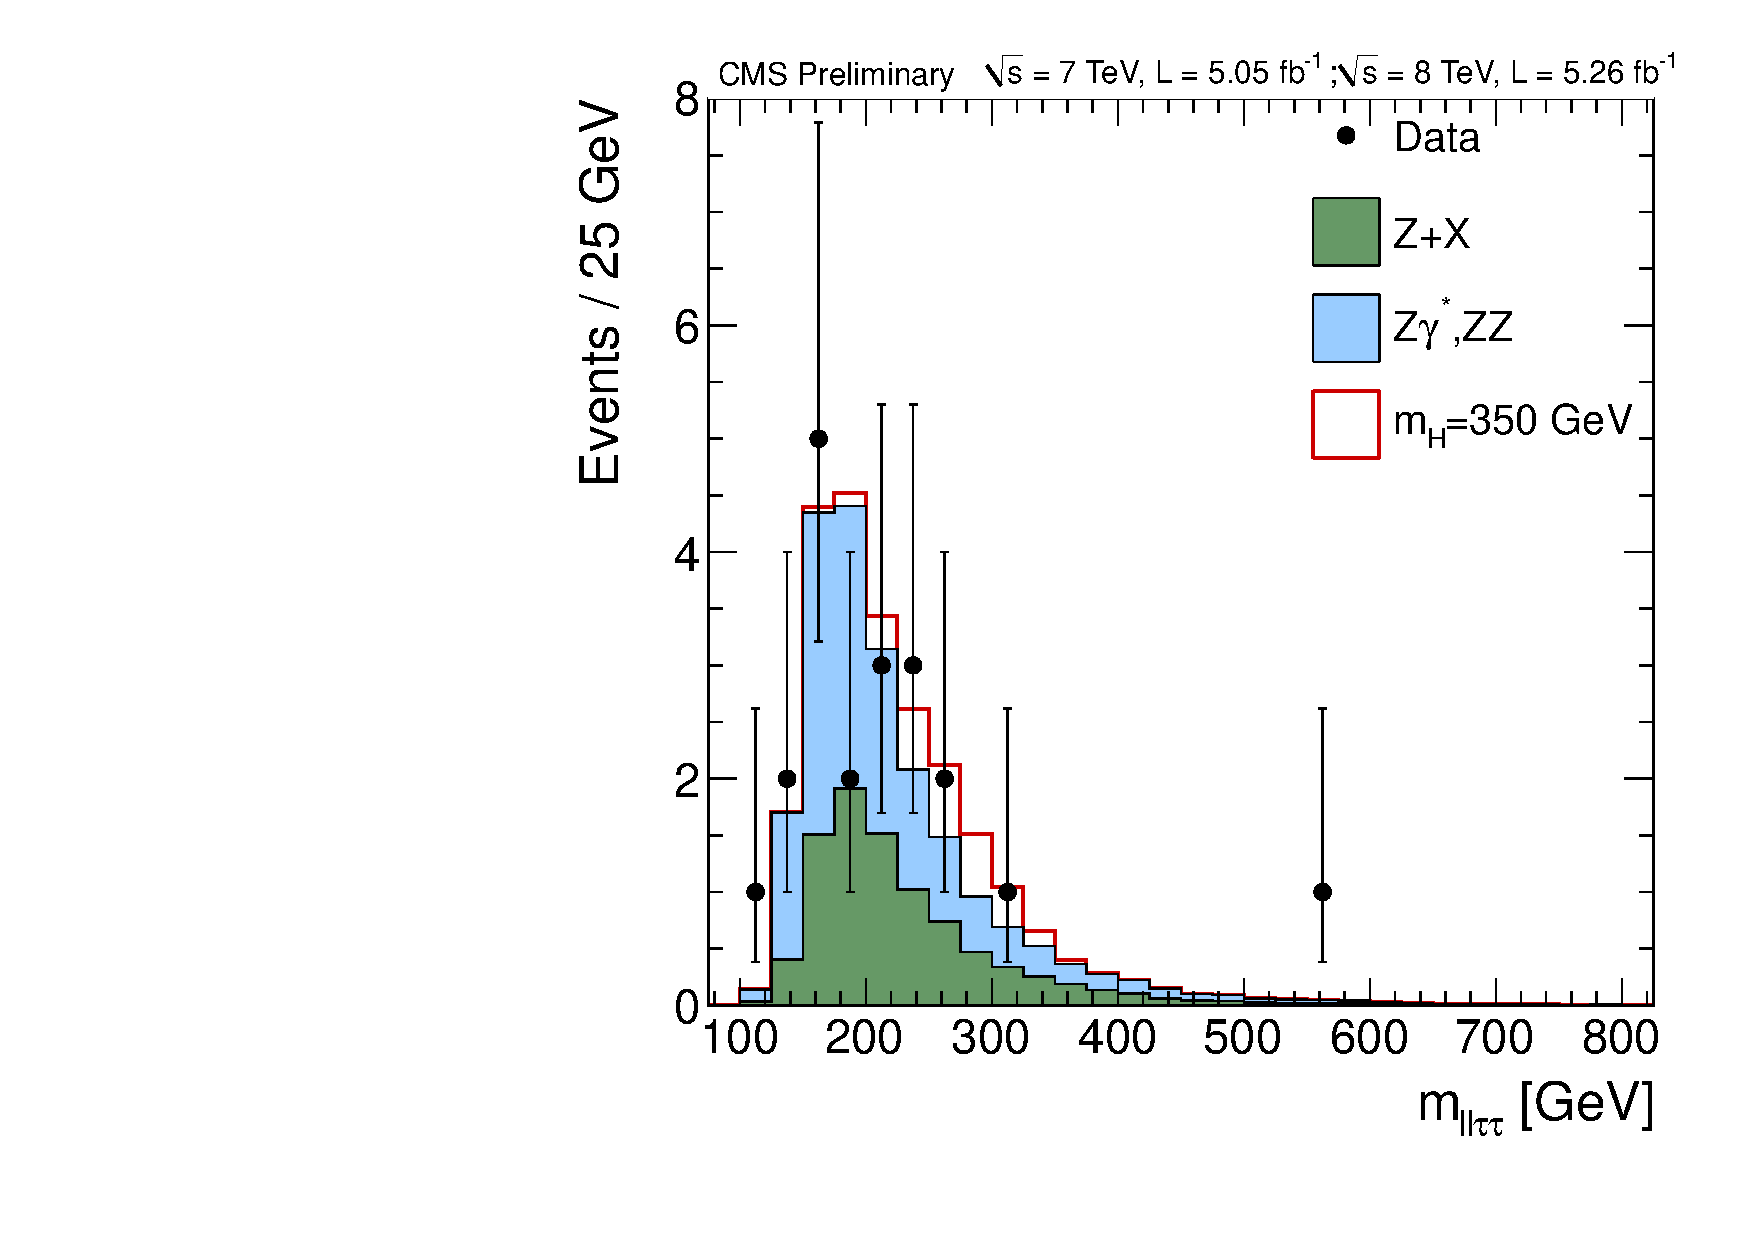
\includegraphics[width=0.4\textwidth]{plots/2l2taumass.pdf}}
\subfigure[]{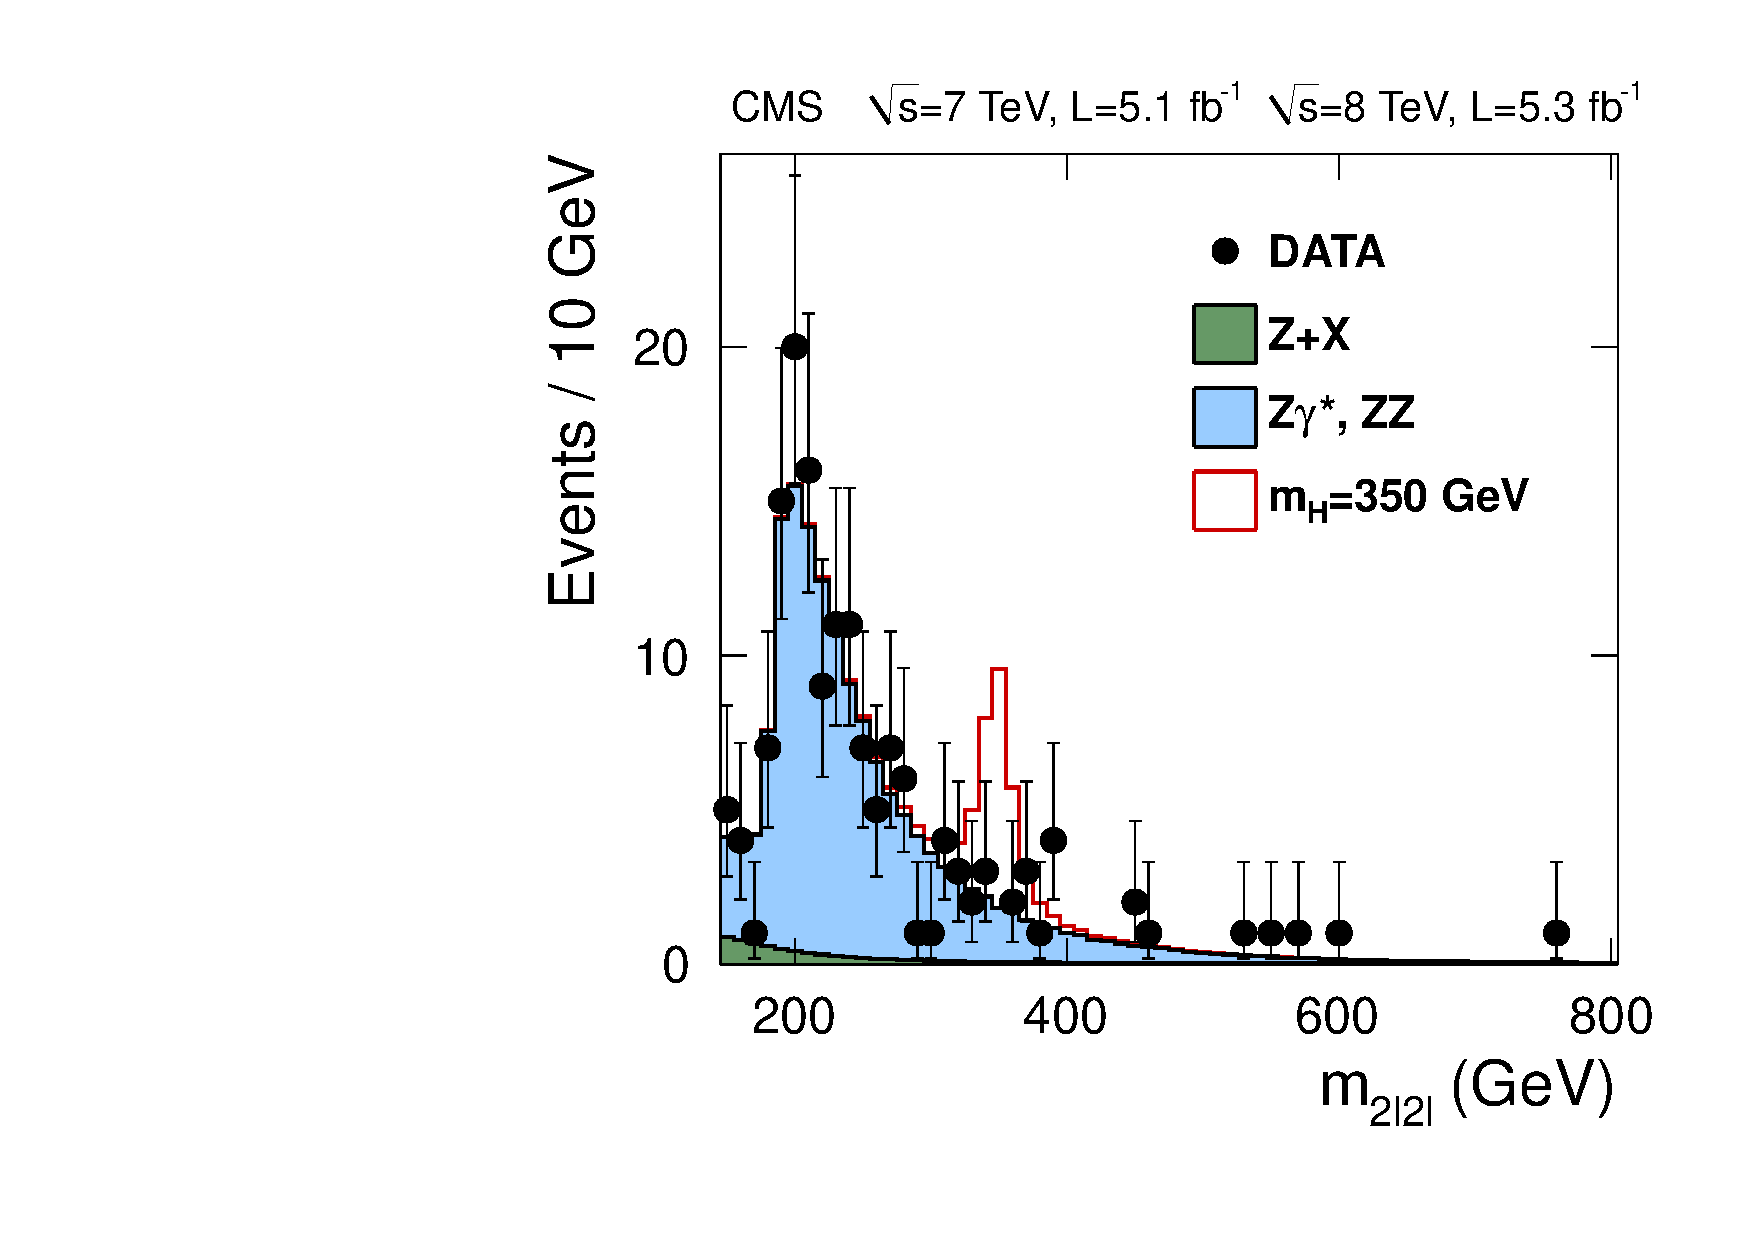
\includegraphics[width=0.45\textwidth]{figures/ZZ4lmass}}
\subfigure[]{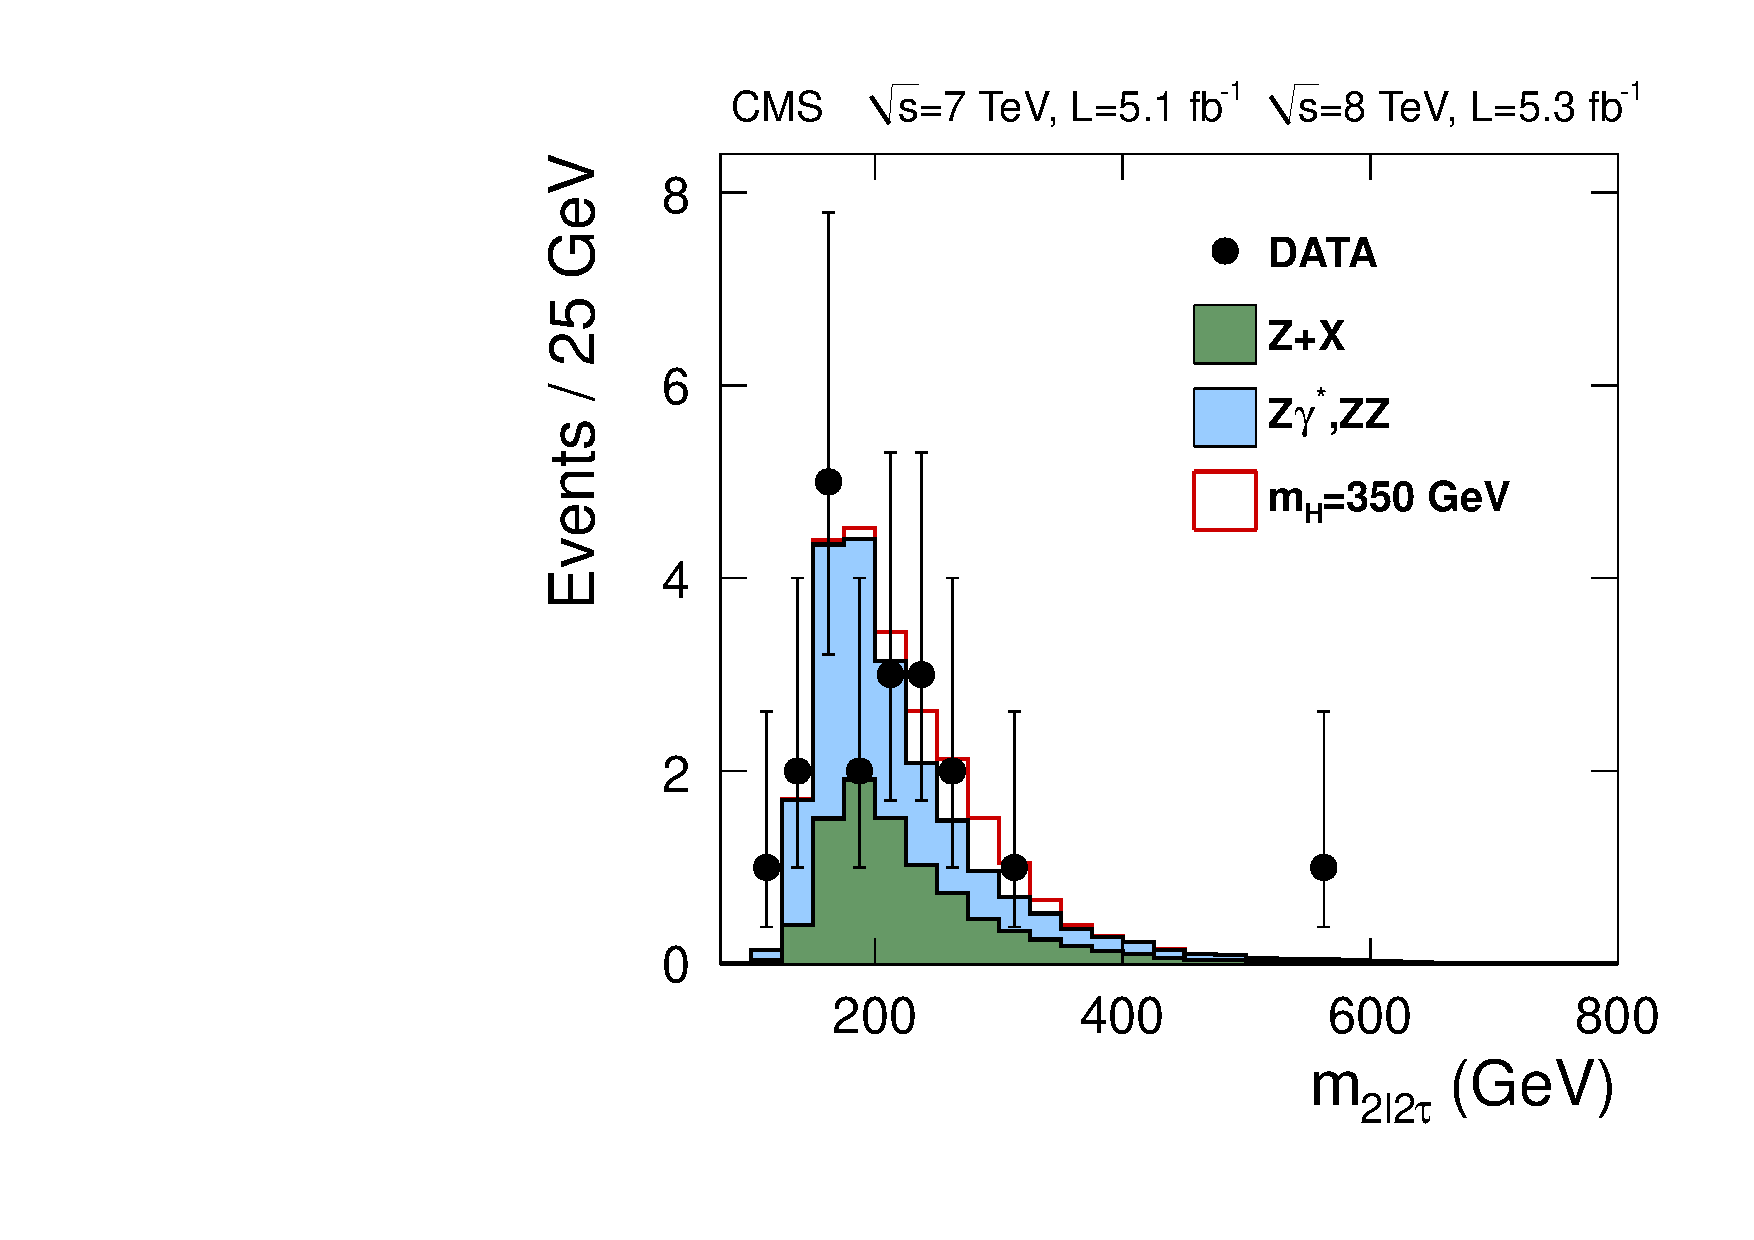
\includegraphics[width=0.45\textwidth]{figures/ZZ2l2tauMass.pdf}}
%
\caption{ 
Distribution of the four-lepton reconstructed mass for (a) the sum of 
the $4\Pe$, $4\Pgm$, and $2\Pe2\Pgm$ channels , and for (b) the sum over all
$2\ell2\tau$ channels .
Points represent the data, shaded histograms represent the background 
and unshaded histogram the signal expectations.
The distributions are presented as stacked histograms.}
\label{fig:Mass4l-2l2tau}
\end{center}
\end{figure}
%=======
The reconstructed visible mass distributions for the $2\ell2\Pgt$ selection, combining all
the $2\ell2\tau$ final states, are shown in Fig.~\ref{fig:Mass4l-2l2tau}(b).
%and compared to SM background expectation. 
The background shapes are taken from MC simulation and the rates are normalised 
to the values obtained using a method based on data.   
The measured distributions are well described by the SM background expectation.

The number of candidates observed in the signal regions 
%as well as the estimated background in the signal region
is reported in Table~\ref{tab:SelectYields}.
%, for the selection in the full mass measurement 
%range for the Higgs boson search.
%,  $160 < m_{4\ell},m_{2\ell2\Pgt}  < 800 \GeV$. 
The expected number of signal events is also given for several Higgs boson mass hypotheses.
The observed event rates for the various channels are compatible with SM background expectation.
%
%=======
\begin{figure}[htbp]
\begin{center}
%
%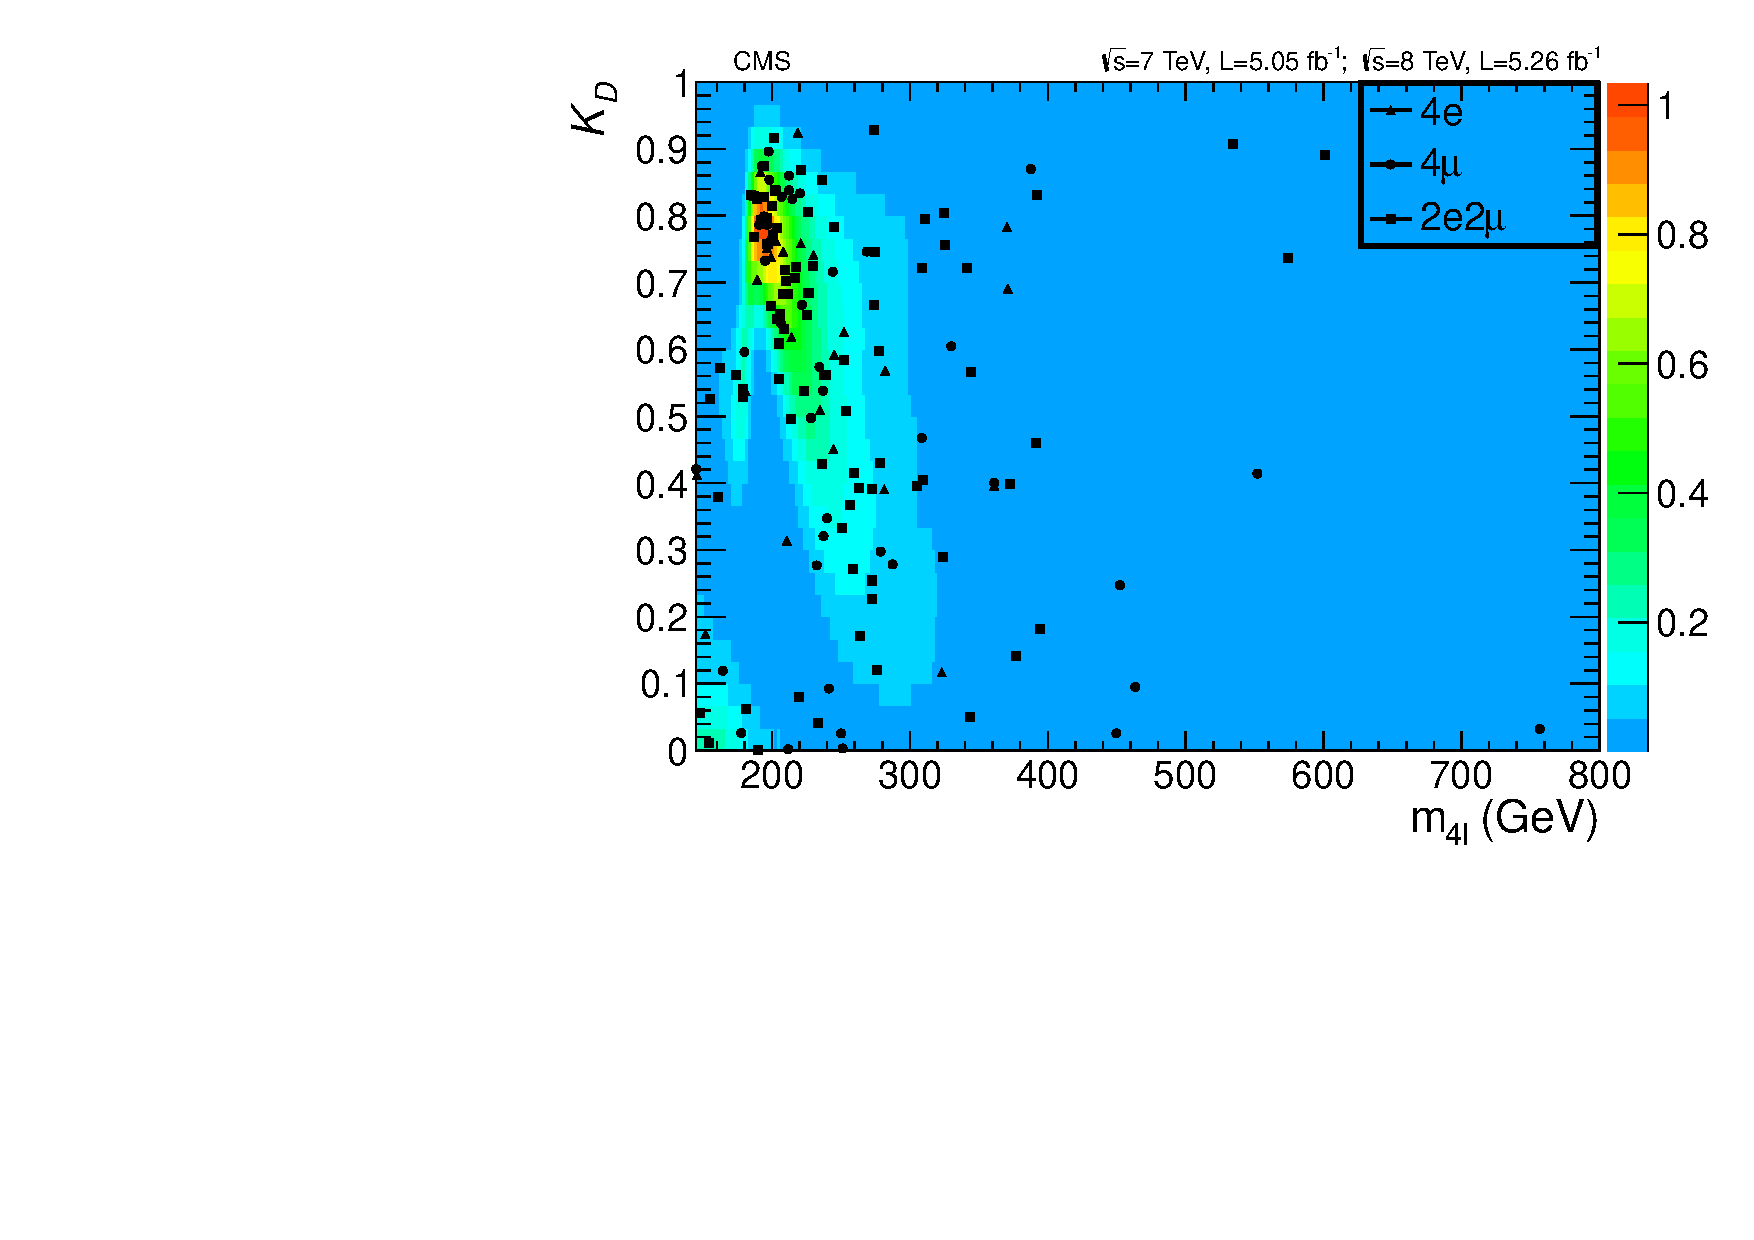
\includegraphics[width=0.5\linewidth]{plots/hzz4lmela.pdf}
%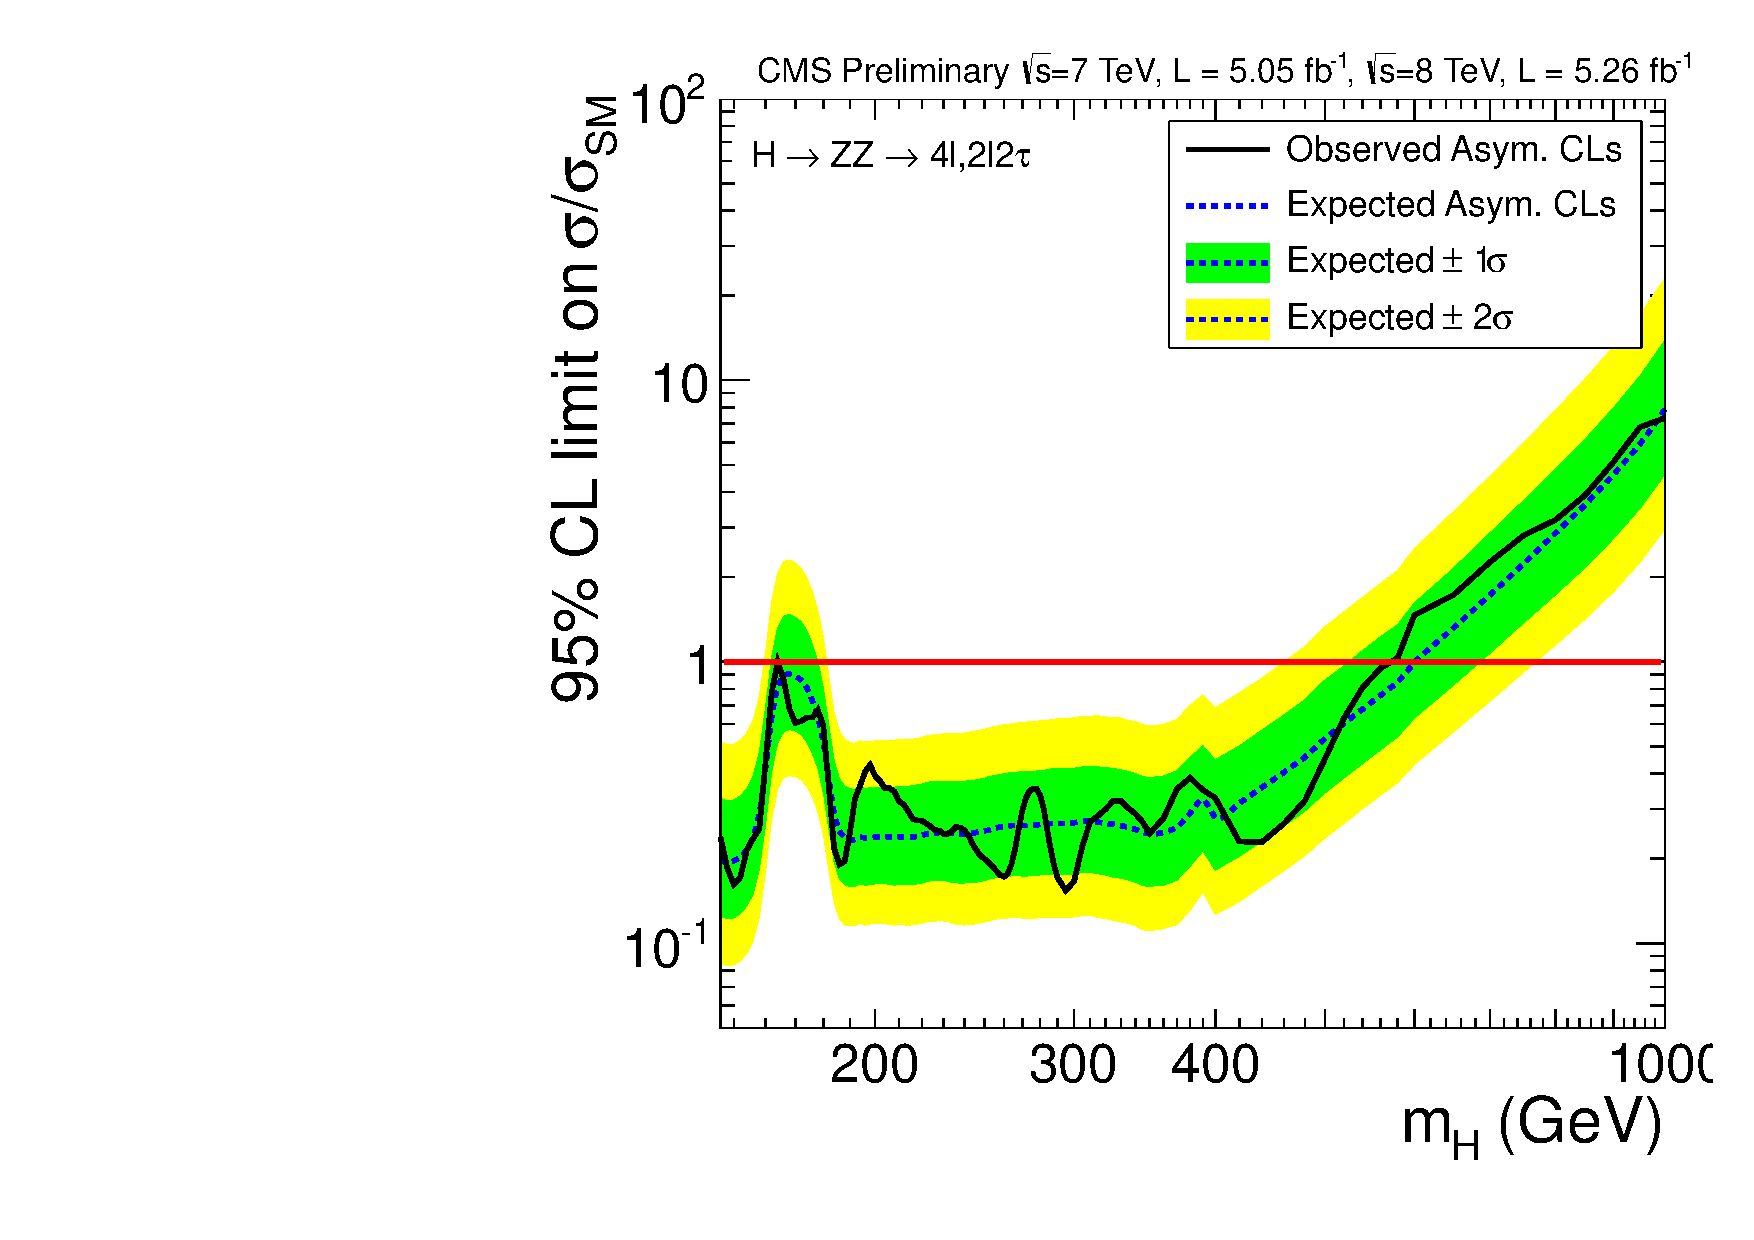
\includegraphics[width=0.4\linewidth]{plots/hzz4llimit7and8TeV.pdf}
\subfigure[]{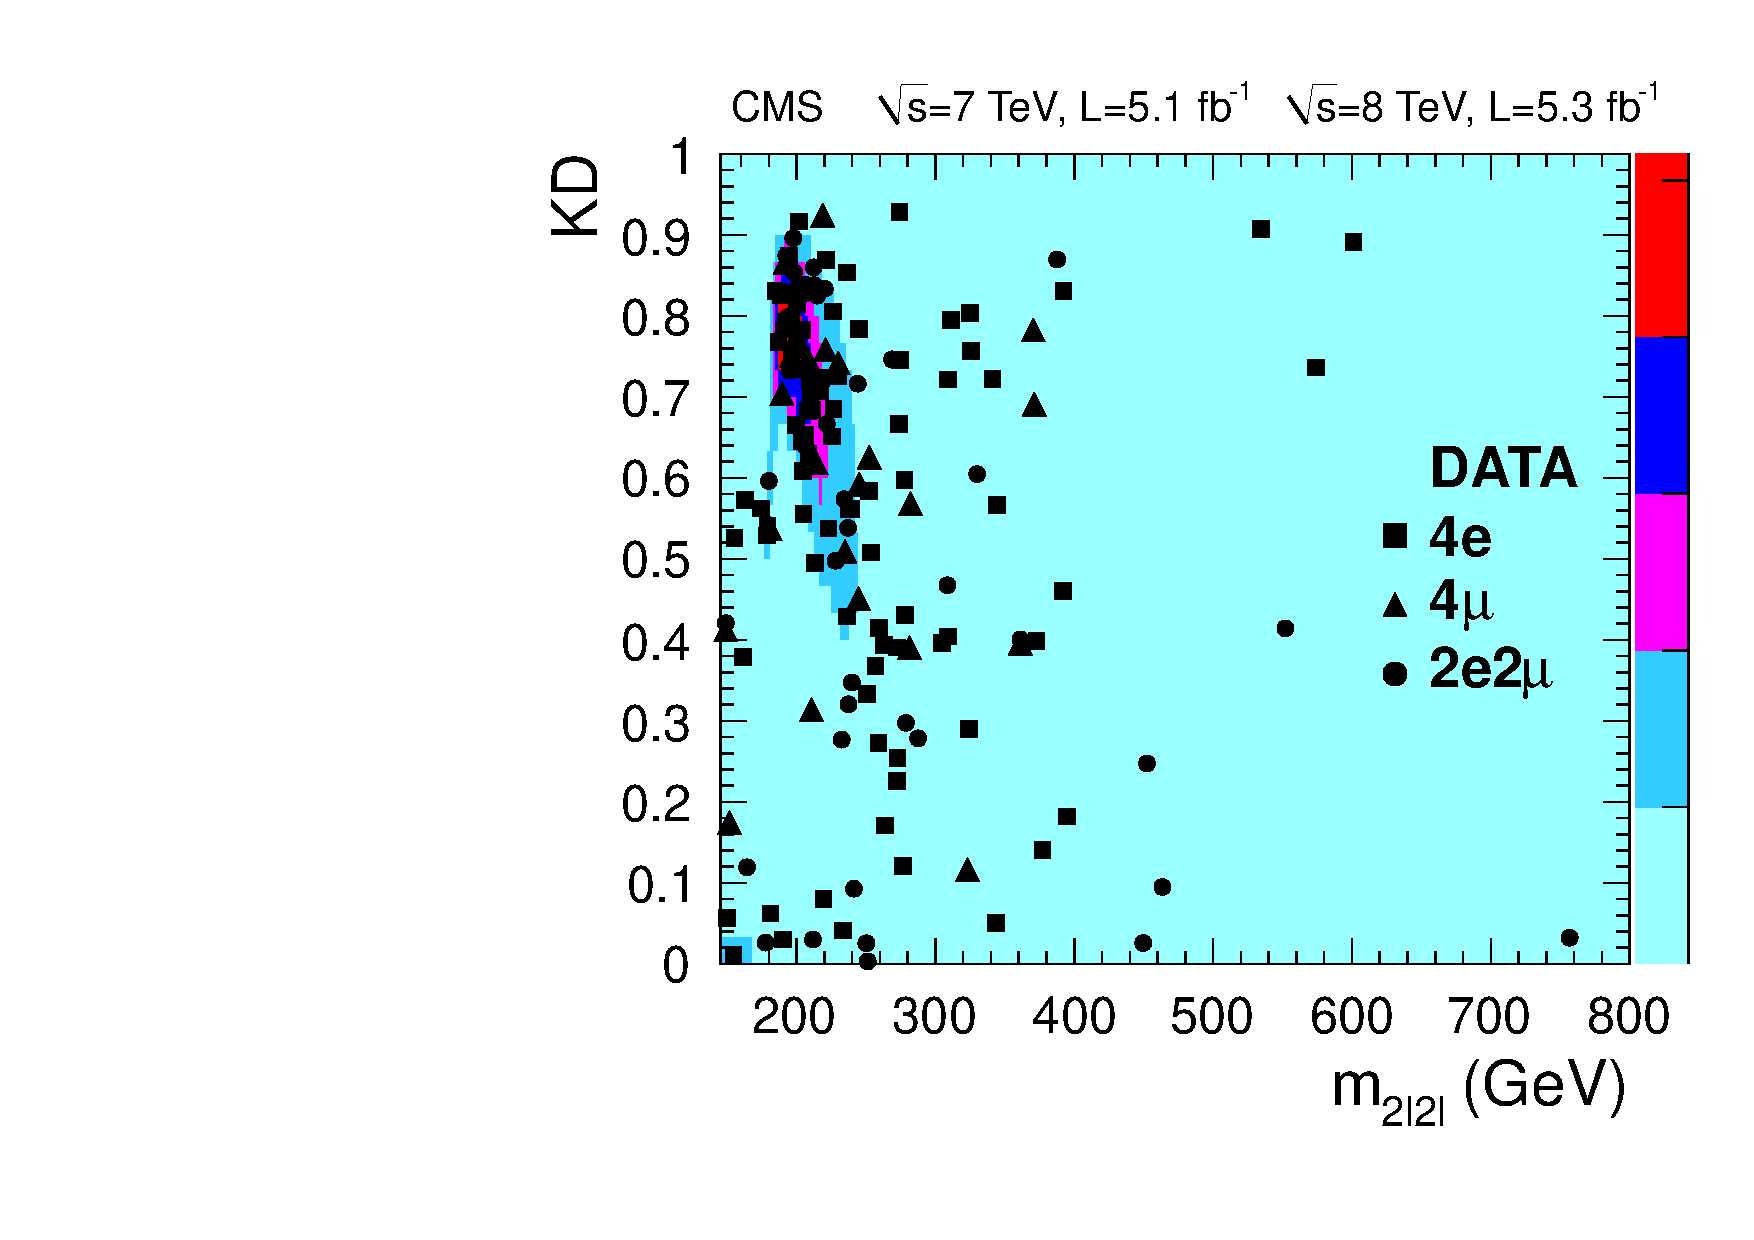
\includegraphics[width=0.45\linewidth]{figures/ZZ4lMELA.pdf}}
\subfigure[]{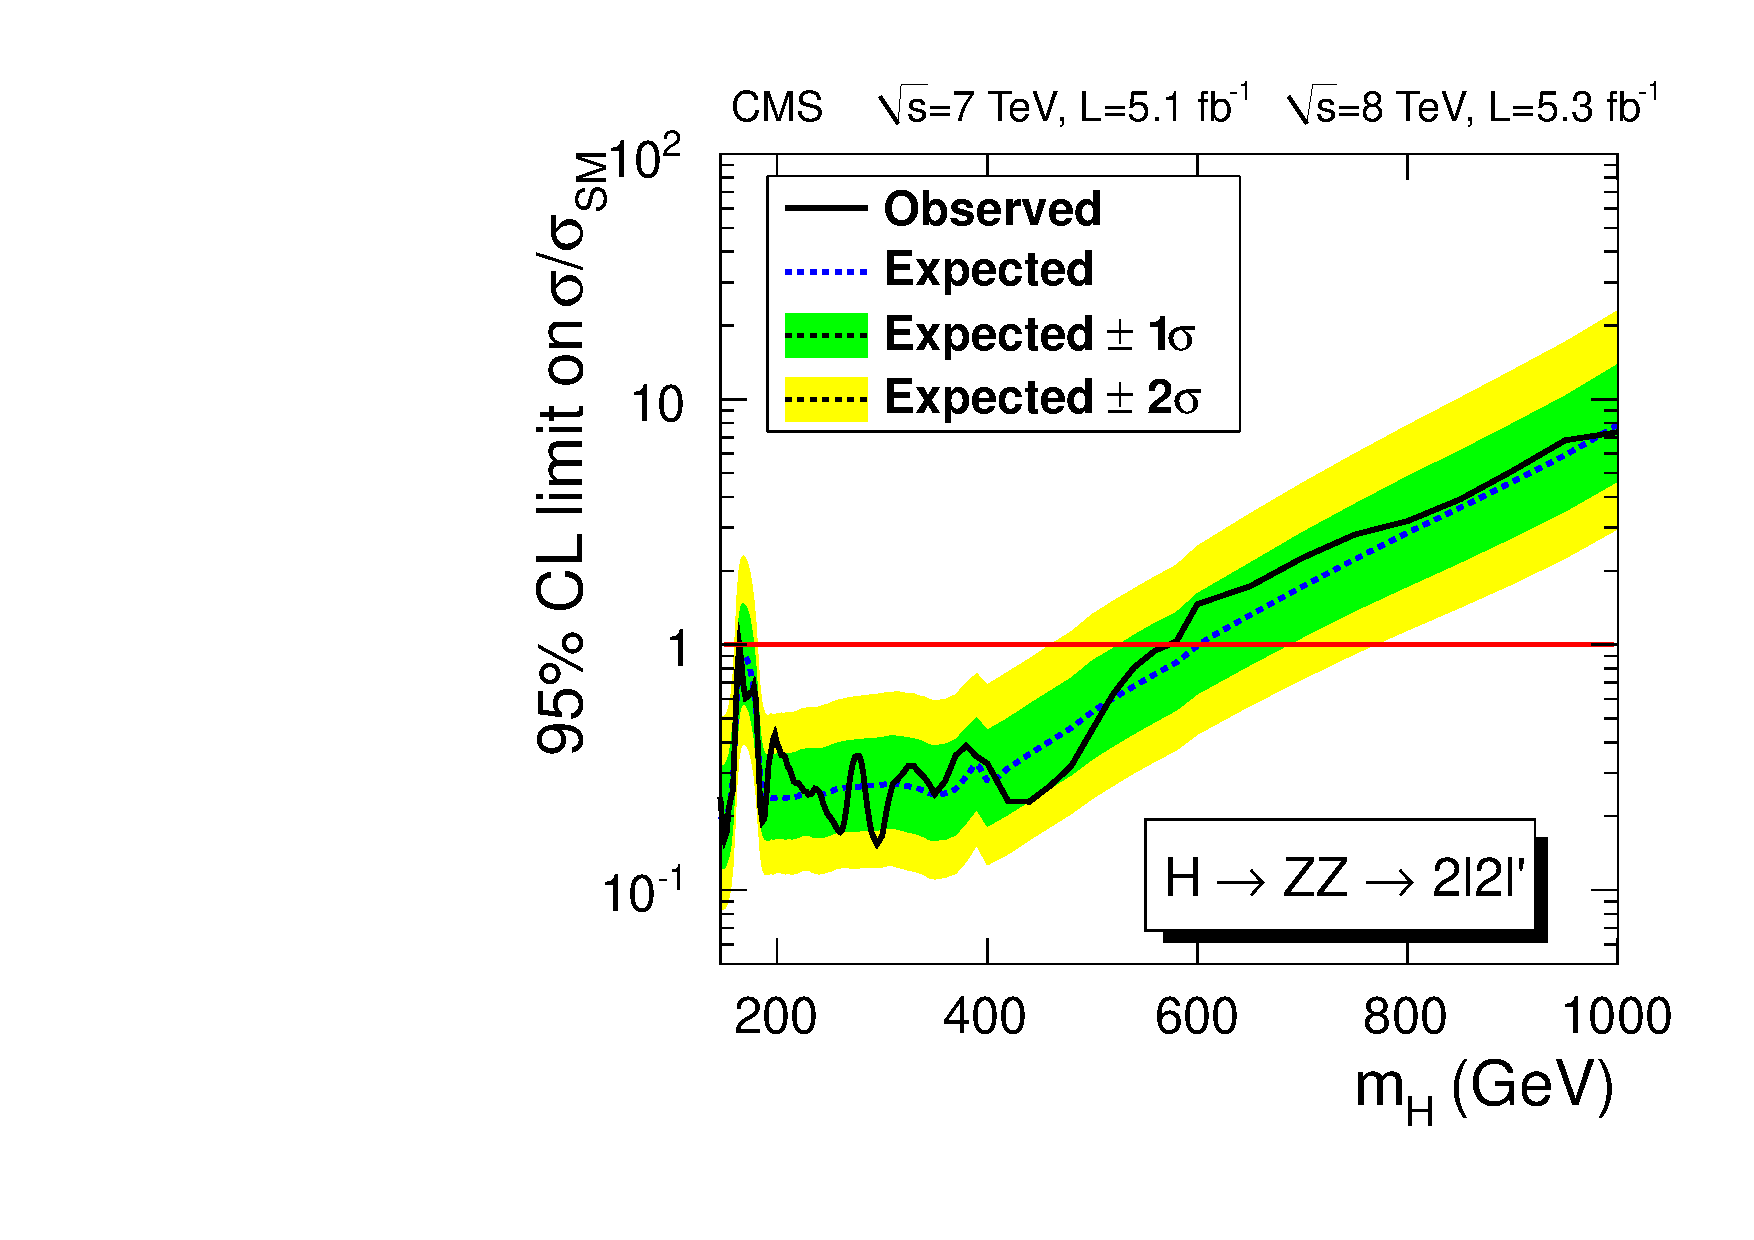
\includegraphics[width=0.45\linewidth]{figures/ZZ4lLimit.pdf}}
%
\caption{ (a) 
The distribution of events
selected in the $2\ell2\ell$ 
subchannels for the kinematic discriminant, KD, versus $m_{4\ell}$.
Events in the three final states are marked by filled symbols (defined in the legend).
%The horizontal error bars indicate the estimated mass resolution.
The contours represent the expected relative density of background events.
(b) Observed and expected 95\% CL upper limit on the ratio of the production cross section to the 
SM expectation.
The 68\% and 95\% ranges of expectation  for the background-only model 
are also shown with green and yellow bands, respectively.
}
\label{fig:KDvsM4lFullMass}
\end{center}
\end{figure}
%=======

The kinematics of the $\PH\to\ZZ \to 2\ell2\ell$ process,
for a given invariant mass of the four-lepton system,
is fully described by five angles and the invariant masses of the two lepton pairs~\cite{Cabibbo:1965zz,Gao:2010qx,DeRujula:2010ys}.
These seven variables provide
significant discriminating power between signal and background.
A kinematic discriminant (KD) is constructed based on the probability ratio of the signal and background hypotheses,
as described in Ref.~\cite{2l2qpaper}.
The distributions of the $\KD$ versus the four-lepton reconstructed mass $m_{2\ell 2\ell}$
is shown for the selected events and compared to SM background expectation 
in Fig.~\ref{fig:KDvsM4lFullMass}(a).
The distribution of events in the $(m_{2\ell 2\ell}, \KD)$ plane is seen to agree well with the 
SM expectation.
%Considering high values of the $\KD\ > 0.5$, three events are observed  
%in the range $520 < m_{2\ell 2\ell} < 600 \GeV$. 

%The probability distribution of ${\cal P}(m_{4\ell})$ for the background is parametrised with empirical 
%functions using MC simulation for $\Zo\Zo$ background and data control regions for  $\Zo+\X$ background.
%The reconstructed signal $m_{4\ell}$ distributions are described with a relativistic Breit-Wigner 
%parametrization convoluted with a Crystal-Ball function~\cite{CrystalBall}. 

%For the $2\ell2\Pgt$ channels, signal and background 
%shape templates are taken from simulation, with the background yields normalised to the 
%data-driven yields described above. 

The two dimentional shape of KD distribution  as a function of $\m_{2\ell2\ell}$ is used to set the upper
limits in $2\ell2\ell$ case. For $2\ell2\tau$ final states the limits are set using the shape of the 
$m_{2\ell2\tau}$ distribution.
The upper limits obtained from the combination of all the $2\ell 2\ell'$ channels
are shown in Fig.~\ref{fig:KDvsM4lFullMass}.
%The SM Higgs boson is excluded at 95\% CL 
%in the range 131--525\GeV.
%, except for the small range 162--172\GeV where the branching
%ratio for the $\PH \rightarrow \cPZ\cPZ$ decay is disfavoured. 

\subsection{$\mathrm{H} \to \ZZ \to 2\ell \mathrm{q\bar{q}}$}

The events are selected by the triggers that require the presence of a
pair of electrons, or a pair of muons. Single electron (muon) triggers are
also used, but their inclusion has almost no impact on the 
efficiency of the event selection.
%We search for a fully reconstructed decay chain of the Higgs boson
%where the charged leptons $\ell^\pm$ are either muons or
%electrons and the quarks are identified as jets in the CMS detector.
Both reconstructed electrons and muons are required to have \PT
greater than 40\GeV and 20\GeV
for the leading and subleading \PT lepton, respectively.
Leptons are measured in the pseudorapidity range $|\eta|<2.5$ for electrons,
and $|\eta|<2.4$ for muons, although for electrons
the transition range between the barrel and endcap, $1.44<|\eta|<1.57$, is excluded.
%Both the $\PT$ and $\eta$ requirements are consistent with those in the online
%trigger selection requiring two charged leptons, either electrons or muons.
%In the high-mass analysis, we also accept events selected with a single-muon trigger.
All jets are required to have $\PT>30\GeV$ and $|\eta| < 2.4$.
Current anlysis uses the same data sample and selections as the published one~\ref{Chatrchyan:2012ft},
but uses most recent Higgs mass line shape reweighting. Therefore we give here 
just a brief description of the selection requirements.

Each pair of oppositely charged leptons of the same flavor and each pair of jets 
are considered as $\Zo$ candidates.
The requirement $75<\mjj<105\GeV$
and $70<\mll<110\GeV$ are applied to reduce background contributions.
Events are classified according to the number of selected $b$-tagged jets
into three mutually exclusive categories:
0 \cPqb, 1 \cPqb\ and 2 \cPqb-tags.  
An angular likelihood discriminant is used to separate signal-like from background-like
events in each category
as described in Ref.~\cite{Gao:2010qx}. 
A "quark -- gluon" likelihood discriminant (qgLD) that separates gluon and light-quark jets 
on a statistical basis is applyed in 
0 \cPqb-tag category, which is dominated by the $\Zo$+jets background.
In order to suppress the substantial $\ttbar$ background in the 2 \cPqb-tag category,
we construct a discriminant, $\lambda$, which is the ratio of the likelihoods of the hypothesis
with $\MET$ equal to the value measured with the PF algorithm and the null
hypothesis ($\MET=0$)~\cite{Chatrchyan:2011tn}.
This discriminant provides a measure that the event contains genuine \MET.
Events in the 2 \cPqb-tag category are required to have
$2\ln{\lambda} (\MET) < 10$. 
When an event contains multiple candidates passing the selection requirements,
we retain the one with jets in the highest \cPqb-tag category for the analysis.
Further ambiguity between multiple candidates is resolved selecting the candidate
with $\mjj$ and $\mll$ values closest to the $\Zo$ boson mass \mZ{}.

The statistical analysis is based on the invariant mass of the Higgs boson candidate,
$\mZZ$, which is calculated using a fit of the final state four momenta and
applying the constraint that the dijet invariant mass is consistent with the mass of the $\Zo$ boson.
%The distributions of the $\mZZ$ for background and
%data are displayed for the three \cPqb-tag  categories
%in Fig.~\ref{fig:mZZ_kinfit_hiMass}. 
Data containing a Higgs boson signal would have a distinct resonance peak in addition
to the continuum background distribution.

The background distributions are estimated
from the  $\mjj$ sidebands, defined as  $60<\mjj<75\GeV$ and $105 <\mjj<130\GeV$.
In simulation, the composition and distribution of the dominant backgrounds in the sidebands
is similar to that in the signal region, $75<\mjj<105\GeV$.
The distributions derived from data sidebands are measured
for each of the three \cPqb-tag categories and give the normalization of the background
and its dependence on $\mZZ$. 
The results of the sideband extrapolation procedures
%are shown as solid curves in Fig.~\ref{fig:mZZ_kinfit_hiMass}
%and 
are in good agreement with the observed distributions in data.
In all cases, the dominant backgrounds
include $\Zo$+jets with either light- or heavy-flavor jets and top background, both of which
populate the $\mjj$ signal region and the $\mjj$ sidebands.
The diboson background amounts to less than 5$\%$ of the total in the 0 and
1 \cPqb-tag categories and about 10\% in the 2 \cPqb-tag category.
%This diboson background is accounted for by $\alpha(\mZZ)$ in the high-mass range
%and by the $\mZZ$ sideband procedure in the low-mass range.
No significant deviation is observed between the data
and the expectation for background. 
The expected and observed event yields are listed in Table~\ref{table-yields}.

%%%%%%%%%%%%%%%%%%%%%%%%%%%%%%%%%%%%%%%%%%%%%%%%%
\begin{table}[htbp]
\begin{center}
\caption{
Observed and expected event yields.
The expected background is quoted from the $\mjj$ sideband procedure and from simulation (MC).
In the low-mass range, the background is estimated from the
$\mZZ$ sideband for each Higgs mass hypothesis and is not quoted in the table.
The errors on the expected background from simulation include only statistical uncertainties.
}
\label{table-yields}
\begin{tabular}{l|c|c|c}
\hline
Category & 0 \cPqb-tag & 1 \cPqb-tag &  2 \cPqb-tag \\
\hline
Background ($\mjj$ sideband)   & $3041\pm54$  & $3470\pm59$  & $258\pm17$  \\
Background (MC)     & $3105\pm39$  & $3420\pm41$  & $255\pm11$  \\
\hline
Observed  & 3036         & 3454         & 285\\
\hline
\mH=550  \GeV        &  6.5 $\pm$ 1.0  & 6.5  $\pm$ 0.9  & 3.6  $\pm$ 0.8 \\
\hline
\end{tabular}
\end{center}
\end{table}

%%%%%%%%%%%%%%%%%%%%%%%%%%%%%%%%%%%%%%%%%%%%%%%%%
%\begin{widetext}
%%%%%%%%%%%%
%\begin{figure}[htbp]
%\begin{center}
%\subfigure[]{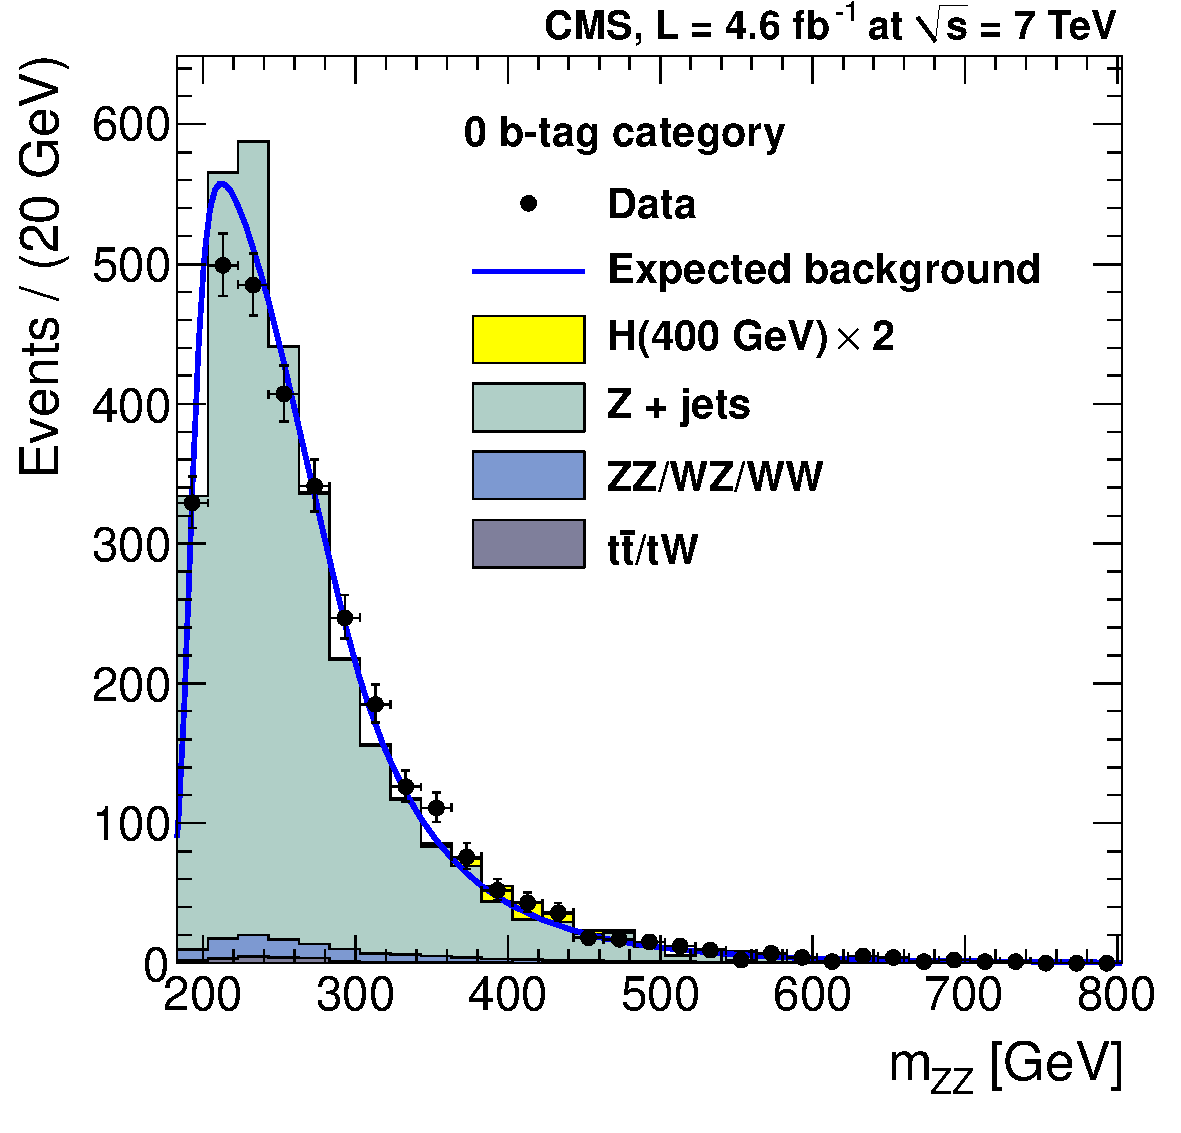
\includegraphics[width=0.3\textwidth]{plots/mzz_0btag.pdf}}
%\subfigure[]{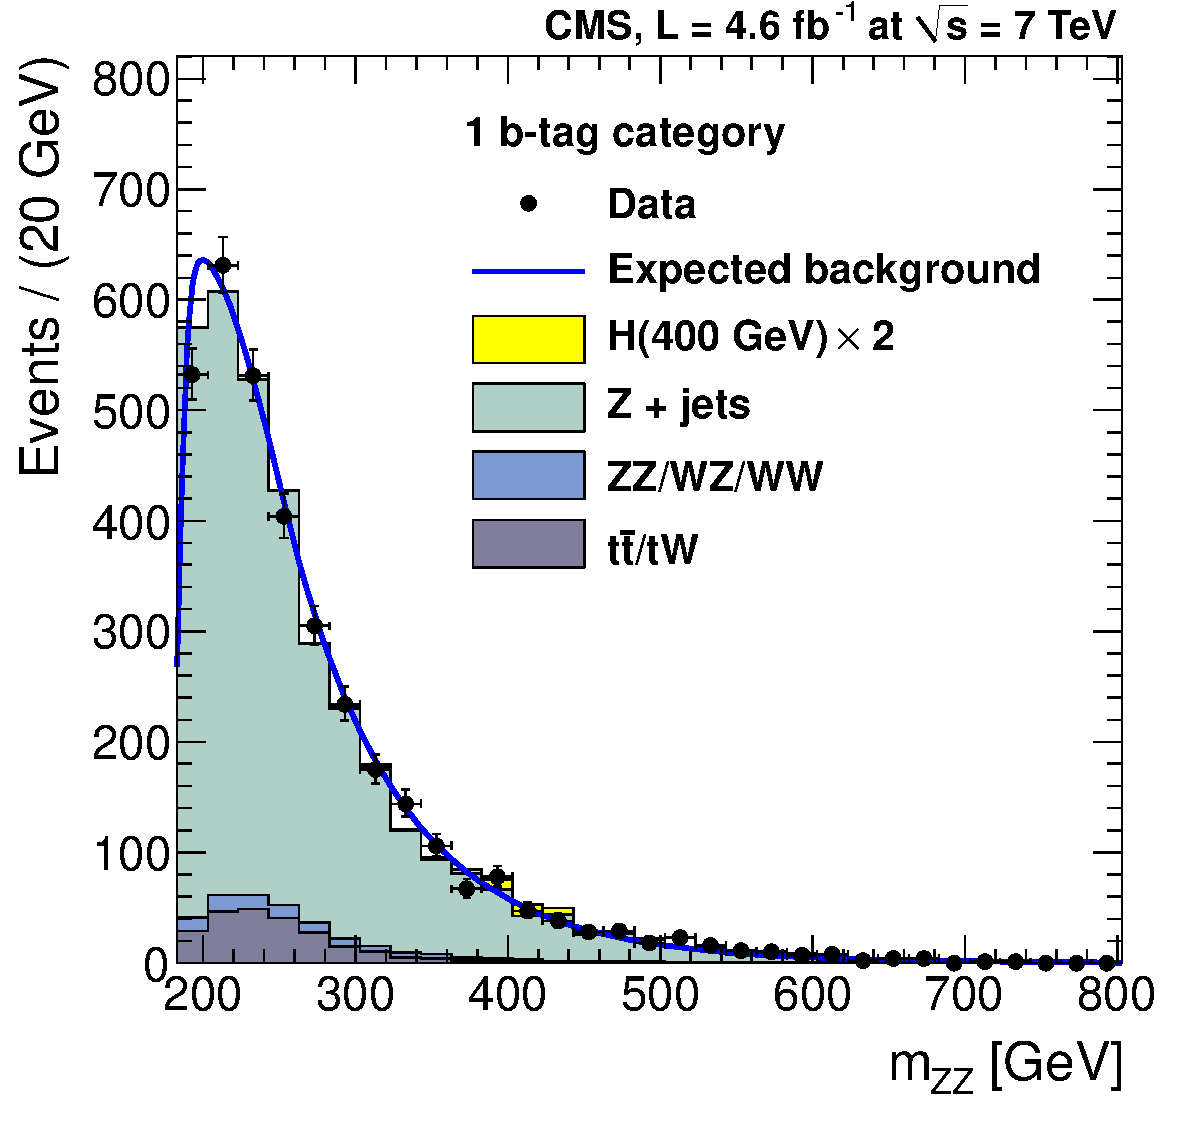
\includegraphics[width=0.3\textwidth]{plots/mzz_1btag.pdf}}
%\subfigure[]{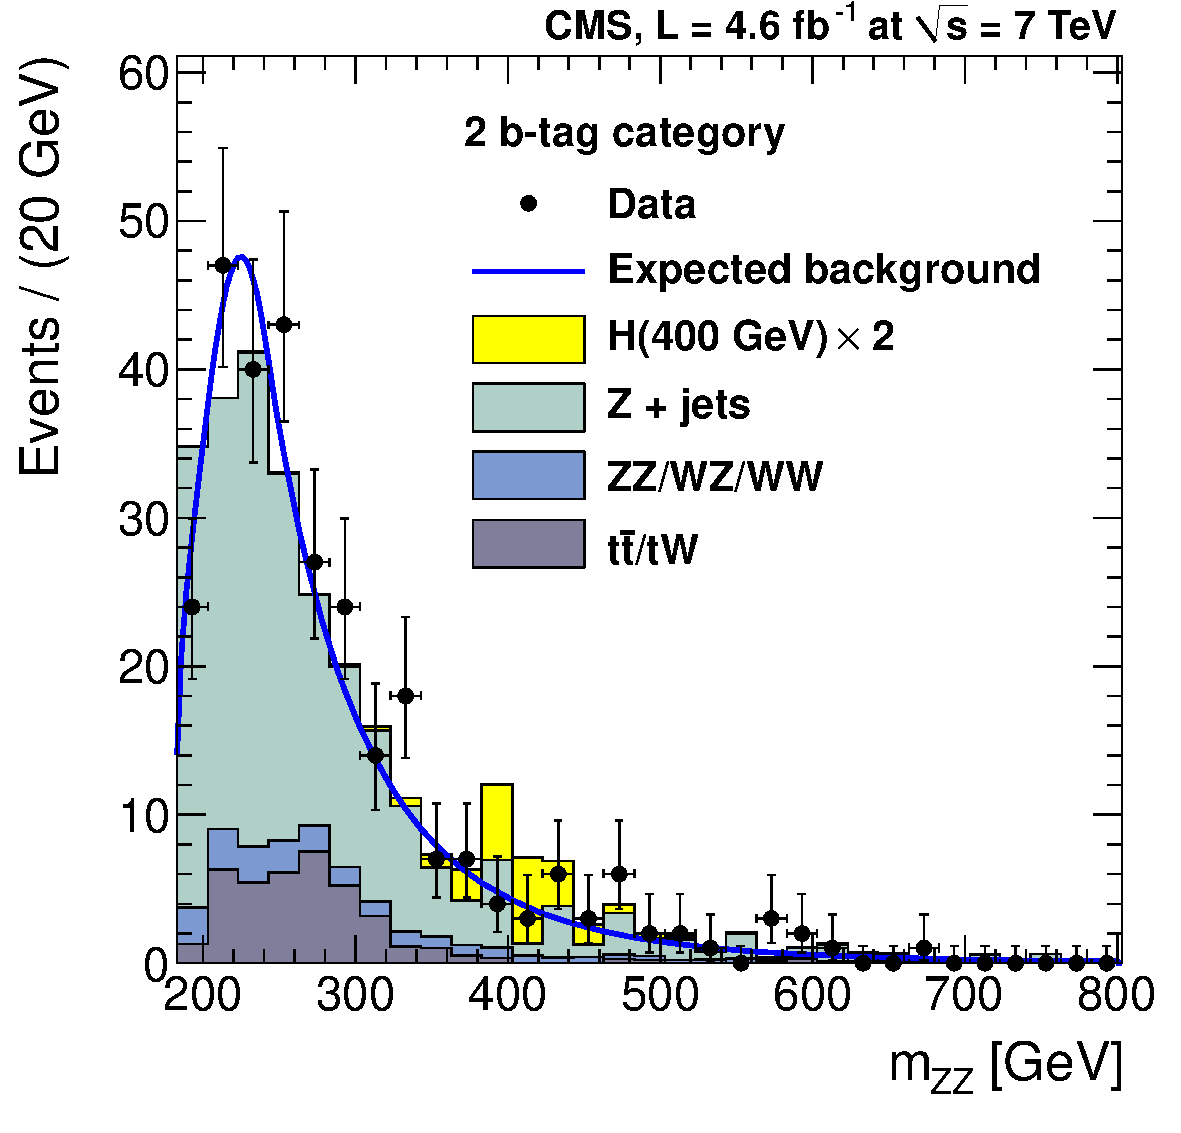
\includegraphics[width=0.3\textwidth]{plots/mzz_2btag.pdf}}
%\caption{
%The $\mZZ$ invariant mass distribution after final selection in three categories:
%(a) 0~\cPqb-tag,
%(b) 1~\cPqb-tag, and
%(c) 2~\cPqb-tag.
%Points with error bars show distributions of data and
%solid curved lines show the prediction of background from the sideband extrapolation procedure.
%In the low-mass range, the background is estimated from the $\mZZ$ sideband for each Higgs
%mass hypothesis and the average expectation is shown.
%Solid histograms depicting the background expectation from
%simulated events for the different components are shown.
%Also shown is the SM Higgs boson signal with the mass of 400\GeV and cross section
%2 times that of the SM Higgs boson, which roughly corresponds to expected exclusion
%limits in each category.
%}
%\label{fig:mZZ_kinfit_hiMass}
%\end{center}
%\end{figure}

\begin{figure}[htbp]
\begin{center}
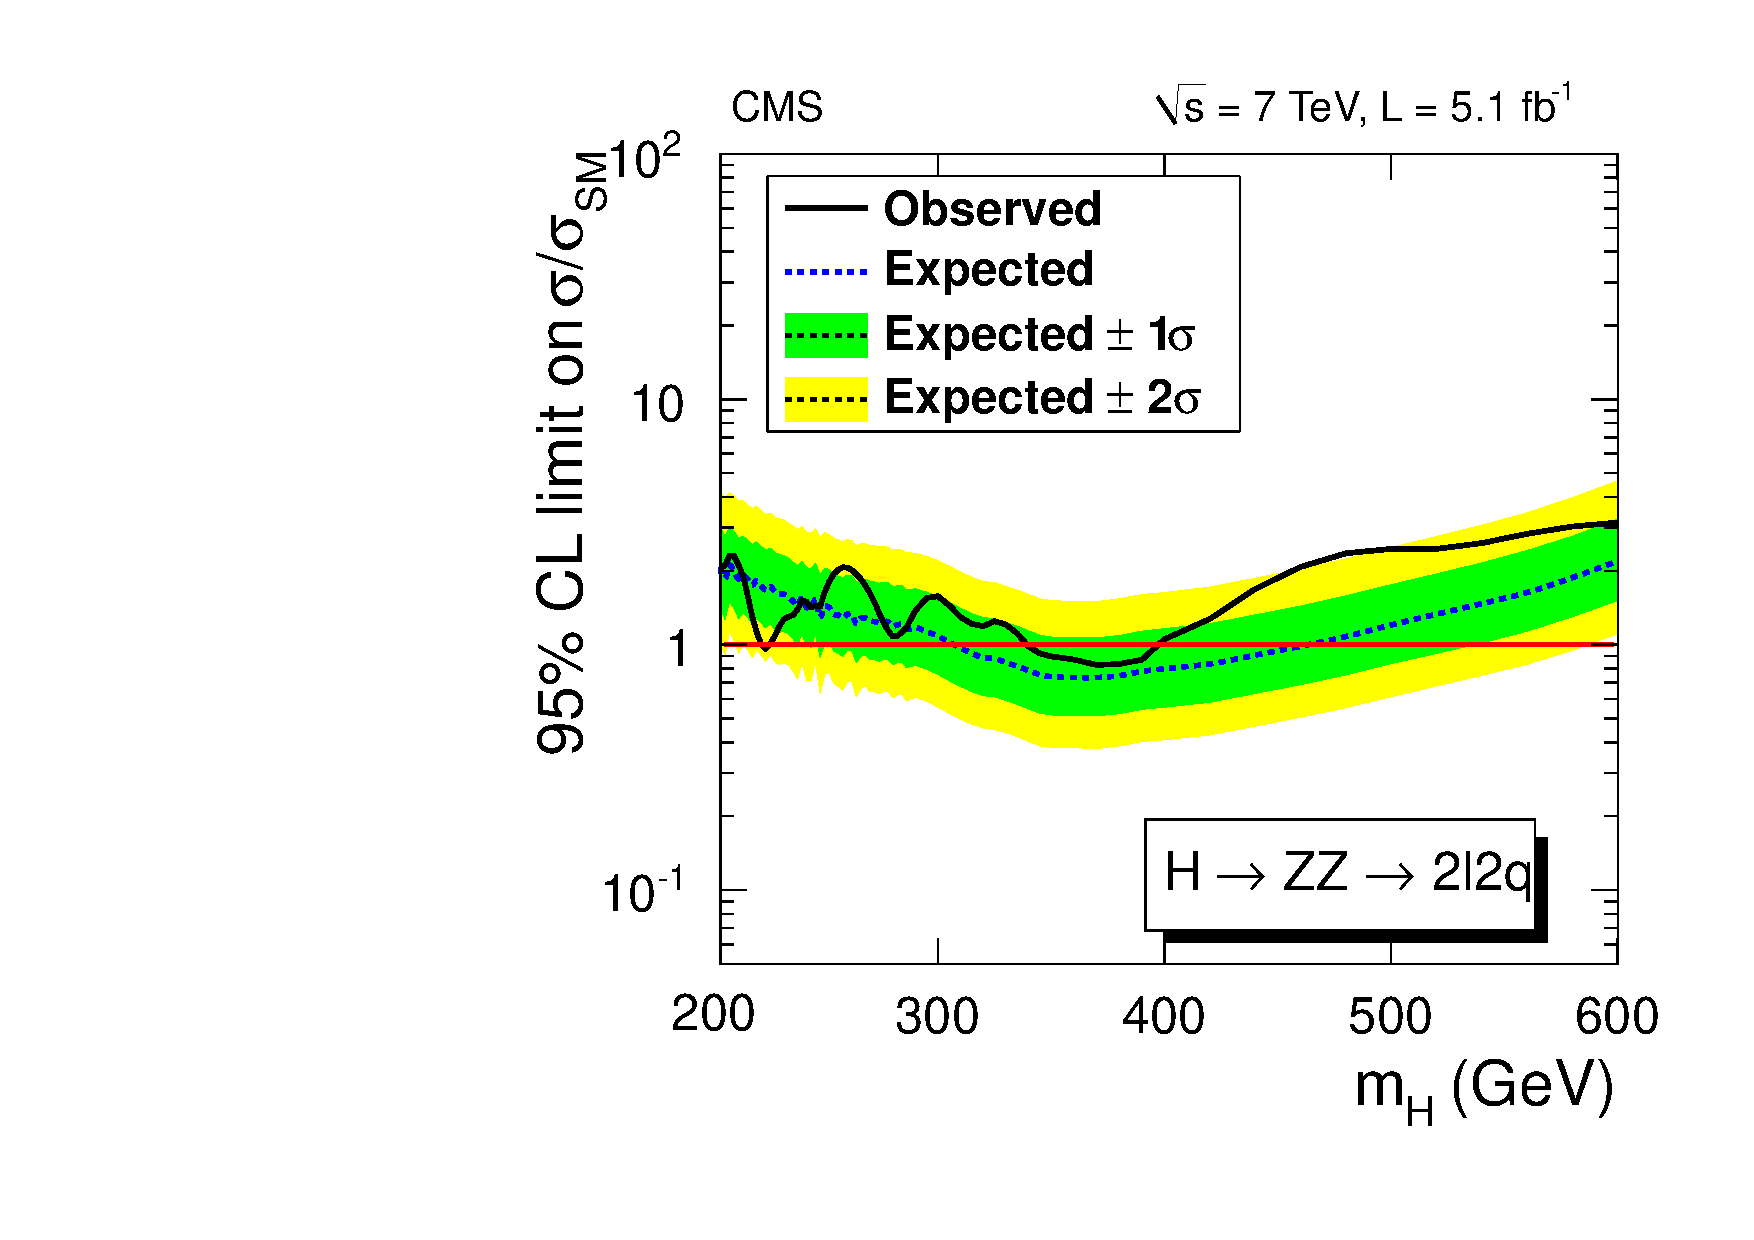
\includegraphics[width=0.6\linewidth]{figures/ZZ2l2qLimit.pdf}
\caption{
Observed (solid) and expected (dashed) 95\% CL upper limit
on the ratio of the production cross section to the SM expectation
for the Higgs boson obtained using the $\mathrm{CL_s}$ technique.
}
\label{fig:ZZ2l2qlimit}
\end{center}
\end{figure}


The distribution of $\mZZ$ for the background is parameterized with an empirical function,
fitted to the shape and normalization determined from the sidebands.
The dominant normalization uncertainty in the background estimation
is due to statistical fluctuations of the number of events in the sidebands.
The reconstructed signal distributions are described with 
a Gaussian function with power-law tails
and an empirical function reflecting misreconstruction of the Higgs boson decay products.
The signal reconstruction efficiency and the $\mZZ$ distribution are parameterized as a function of $\mH$
and are extrapolated to all mass points. The main uncertainties in the signal $\mZZ$ parameterization
are due to resolution which is predominantly affected by the uncertainty on the jet energy scale~\cite{Chatrchyan:2011ds}.
Uncertainties due to \cPqb\ tagging have been evaluated with a sample of jet
events enriched in heavy flavor by requiring a muon to be spatially close to a jet.
The uncertainty on the qgLD selection efficiency was evaluated using the $\Pgg+\text{jet}$
sample in data, which predominantly contains quark jets.
%The observed limits are within expectation for the background-only model.
%The significance of the only local deviation beyond the 95\% expectation range
%around 225\GeV
%is greatly reduced after taking into account the look-elsewhere effect~\cite{LEE},
%for which the estimated trial factor is about 18 in the high-mass range.
%Results obtained with the Bayesian approach yield very similar limits to those from $\mathrm{CL_s}$.

The upper limits 
at 95\% CL on the ratio of the production
cross section for the Higgs boson to the SM expectation is
obtained from the combination of all categories 
is presented in Fig.~\ref{fig:ZZ2l2qlimit}.

\subsection{$\PH \to \ZZ \to 2\ell 2\nu$}

Events are selected to have a pair of well-identified, isolated leptons of same flavour ($\Pep\Pem$ or
$\Pgmp\Pgmm$) with $\PT > 20\GeV$ 
%that have an
with invariant mass within a 30\GeV window centered on the $\cPZ$
mass. The $\PT$ of the dilepton system is required to be greater than
55\GeV.  In the electron channel, the events are collected by using
dielectron triggers, and
the muon channel relies on single- or double-muon triggers.
The analysis strategy is based on selection requirements in the (\MET,\MT)
phase space, where selections are adjusted for different $\mH$ hypotheses. 
A detailed description of the analysis can be found in Ref.~\cite{2l2qpaper}.

%Electron candidates
%with an ECAL cluster in the transition region between ECAL barrel and
%endcap ($1.4442 < |\eta| < 1.566$) are rejected.  
The presence of a large \MET in an event
 is a fundamental feature of the signal.
%A large \MET threshold is imposed to suppress the bulk of the $\cPZ$+jets background,
%which contains little genuine \MET.
%The region of large \MET is populated by $\cPZ$+jets events in which the \MET
%is largely due to mismeasurement of the jet energies.
To suppress $\cPZ$+jets 
background, events are removed if the angle in the azimuthal
plane between the \MET and the closest jet with transverse energy $\ET > 30\GeV$ is
smaller than 0.5 radians. 
In order to remove events where the lepton is mismeasured
we reject events with 
\MET$>$60\GeV in which the \MET direction is
pointing near one of the two leptons in the events, i.e. if $\Delta\phi$($\ell$,\MET)$<0.2$.

We use a $b$-tagging veto to reject the top-quark background.
The top-quark background is suppressed by applying a veto on 
events having a \cPqb-tagged jet with $\ET > 30\GeV$ and
$|\eta| < 2.5$.
To further suppress the top-quark background, a veto is applied on events containing a ``soft muon''
with $\PT > 3\GeV$, which is typically produced in the leptonic decay of a b quark.
%The soft-muon veto along with the \cPqb-jet veto reduces the top-quark background by a factor of six.
To reduce the $\PW\cPZ$ background in which both bosons decay leptonically,
any event with a third lepton ($\Pe$ or $\Pgm$) with $\PT > 10\GeV$ and
passing the identification and isolation requirements is rejected.

We search for the resonant production of $\ZZ$ pairs via a SM-like Higgs decay
by analyzing the spectra of \MET and $m_\mathrm{T}^{\ell\ell,\MET}$.
The search is carried out in two mutually exclusive categories. 
VBF category, with two or more jets in the forward region,
with a $|\Delta\eta|>4$ between the two closest jets, and a minimal
invariant mass of those two jets of 500 \GeV. 
In addition the two leptons forming the \cPZ\ 
candidate are required to lie in between these two jets, while no other
selected jets are allowed in this central region. 
The gluon fusion category includes all events failing the VBF selection and is
subdivided into subsamples according for the presence or absence of reconstructed jets with $\PT>$30~\GeV. 
The event categories are chosen such that the best expected limit is
achieved.


%The so-called two jets category is inclusive of all higher jet multiplicities.

The Higgs boson search is performed by
looking for an excess of events above the SM background
expectation after applying selection criteria on
the $\MET$ and $m_\mathrm{T}^{\ell\ell,\MET}$, that are tuned for a
given Higgs-boson-mass hypothesis. 
%The \MET and $\MT$ selection
%listed in Table~\ref{tab:met_mtcuts} was optimized based on the expected limits. 
%The optimization was performed on nine $\mH$ points, and a smooth-fit interpolation for the 
%values of the kinematic requirements was performed to provide optimal values for every explored Higgs mass point.
In case of the VBF category 
a constant $\MET>70\GeV$ and no $m_\mathrm{T}^{\ell\ell,\MET}$ 
requirement are used as no gain in sensitivity is obtained with a 
Higgs-mass-dependent selection.


%\begin{table}[htbp]
%\caption{
%      Higgs boson mass-dependent selection for \MET and
%      $\MT$ variables in the 
%      %and shape-based 
%      gluon fusion analysis.}
%\begin{center}
%\begin{tabular}{c|ccccc}\hline
%$\mH$ (\GeVns)    & 200        & 300        & 400         & 500        & $\geq$600 \\
%\hline
%\hline
%\MET (\GeVns)     & $>75$     & $>85$     & $>90$      & $>90$     & $>100$  \\
%$M_T$ (\GeVns)    & $175 - 275$ & $250 - 375$ & $325 - 450$  & $400 - 650$ & $450 - \infty$ \\
%\hline
%\end{tabular}
%\end{center}
%\label{tab:met_mtcuts}
%\end{table}

The background composition varies with $\mH$. While at low $\mH$ $\cPZ$+jets and
$\ttbar$ contribute the most, at higher $\mH$ (above 400 GeV) the irreducible $\ZZ$ and $\PW\cPZ$ backgrounds are dominating.
The $\cPZ\cPZ$ and $\PW\cPZ$ backgrounds are taken from the MC simulation and are
normalized to their respective NLO cross sections. 
%The remaining backgrounds are
%estimated using control samples in data.
The $\cPZ$+jets background is modeled from an orthogonal control sample of events
with a single photon produced in association with jets ($\Pgg+\text{jets}$).
%This choice has the advantage of making use of a large statistics sample, 
%which resembles in all aspects the $\cPZ$ production in all important aspects: i.e. production mechanism,
%underlying event conditions, pileup scenario, and hadronic recoil. 
%By using the $\Pgg+\text{jets}$ expectation we avoid the need to use the prediction from simulation
%for the instrumental background arising from the mismeasurement of jets.
%from processes that have a photon
%produced in association with genuine \MET,
%such as $\PW(\ell\cPgn)+\Pgg$, $\PW(\ell\cPgn)$+jets, where the jet is mismeasured as a photon,
%and $\cPZ(\cPgn\cPgn)+\Pgg$ events.
%The kinematics and overall normalization of $\Pgg+\text{jets}$ events
%are matched to $\cPZ+\text{jets}$ in data through an event-by-event
%reweighting as a function of the boson $\PT$ in each of the jet multiplicity bins separately,
%to account for the dependence of the \MET on the associated hadronic activity.
%Residual discrepancies can arise due to differences in the effective pile-up of the $\Pgg+\text{jets}$ sample  
%due to the photon trigger pre-scale and 
%event selection. These are taken into account by reweighting events according to the number of reconstructed vertices.
The procedure yields an accurate model of the \MET distribution in $\cPZ$+jets events,
as shown in Fig.~\ref{fig:zgamma_met_data}, which compares the
\MET distribution of the reweighted $\Pgg$+jets events along with other backgrounds to the \MET
distribution of the dilepton events in data.
%To compute the $\MT$ for each
%$\Pgg$+jets event, the value of $\vec{p}_\mathrm{T}(\ell\ell)$ is defined as the photon $\vec{p}_\mathrm{T}$
%and the value of $M(\ell\ell)$ is chosen according to a probability density function
%constructed from the measured dilepton invariant mass distribution in $\cPZ$+jets events.
\begin{figure}[htbp]
\begin{center}
%\subfigure[]{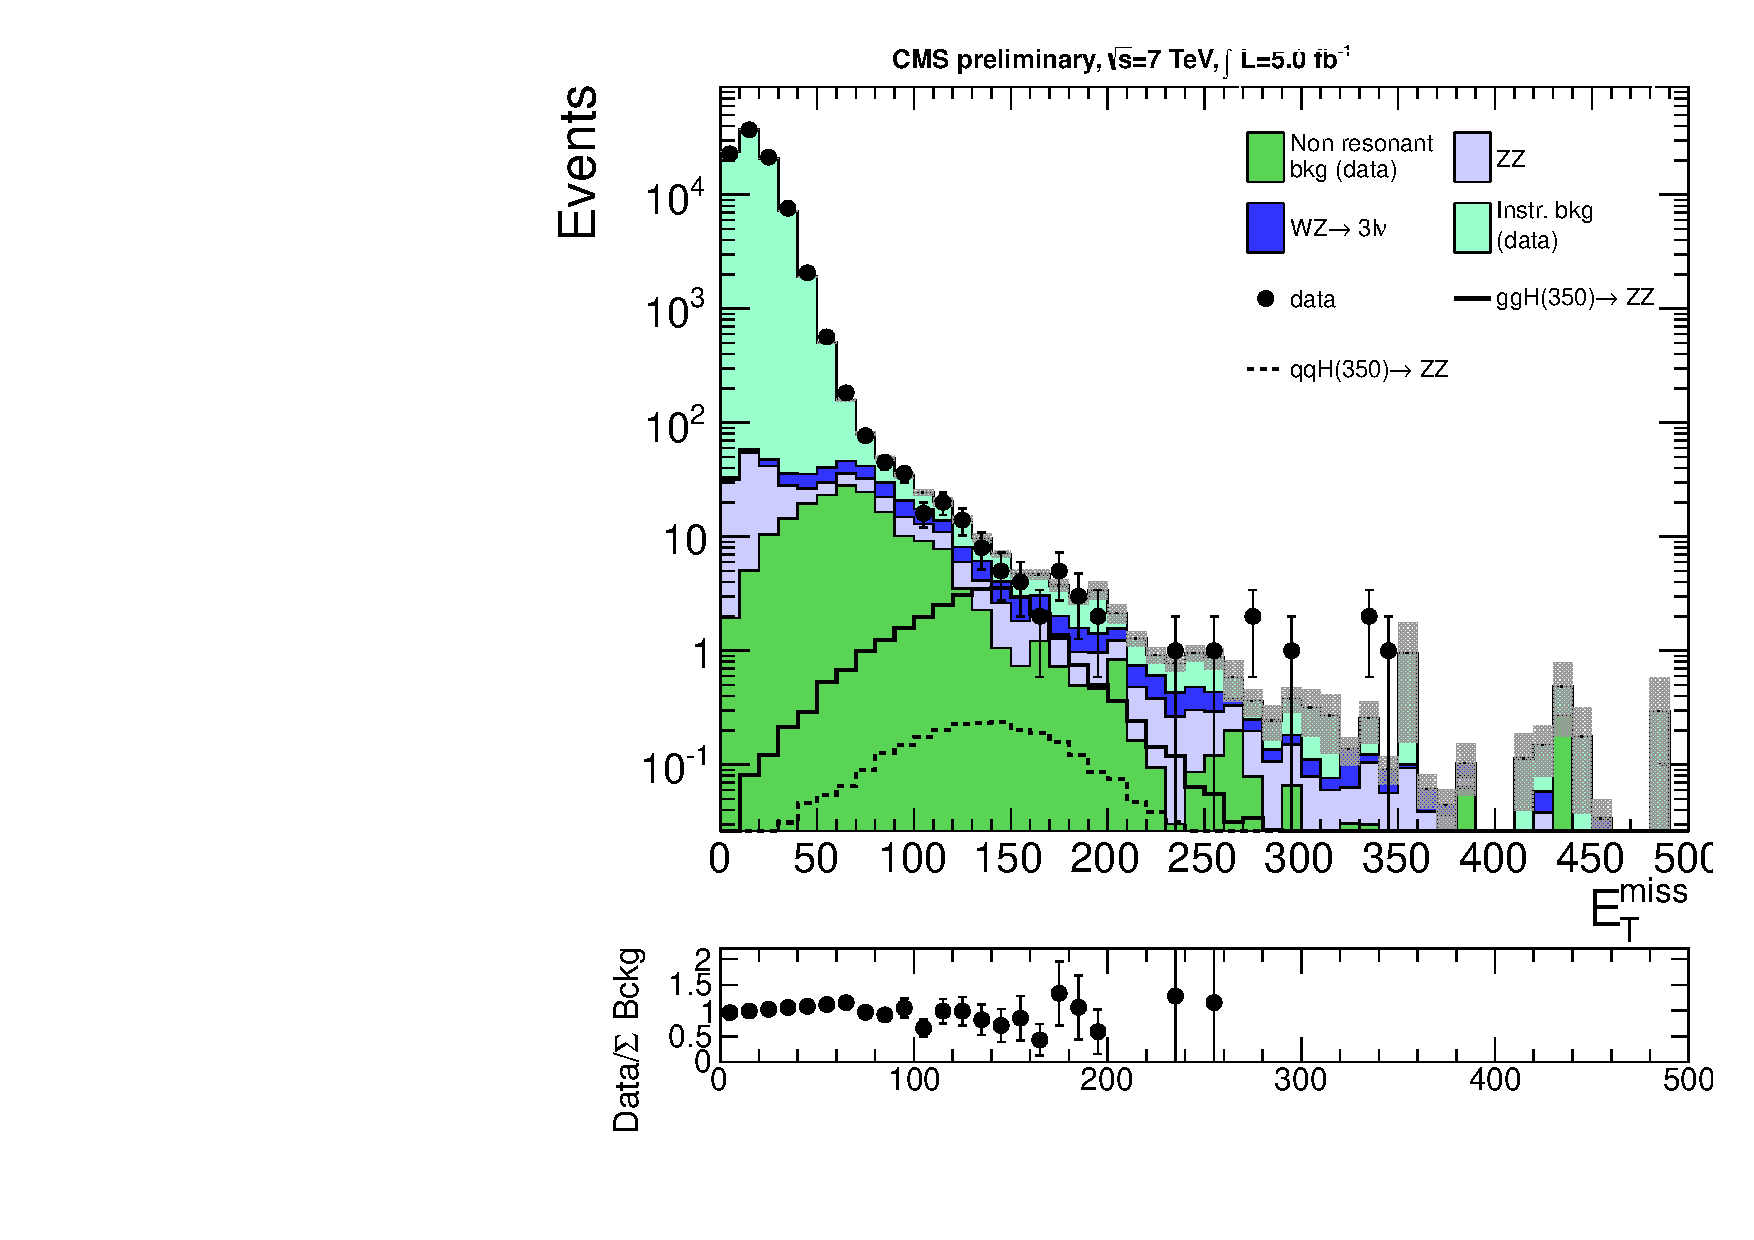
\includegraphics[width=0.48\textwidth]{plots/met_7TeV.pdf}}
%\subfigure[]{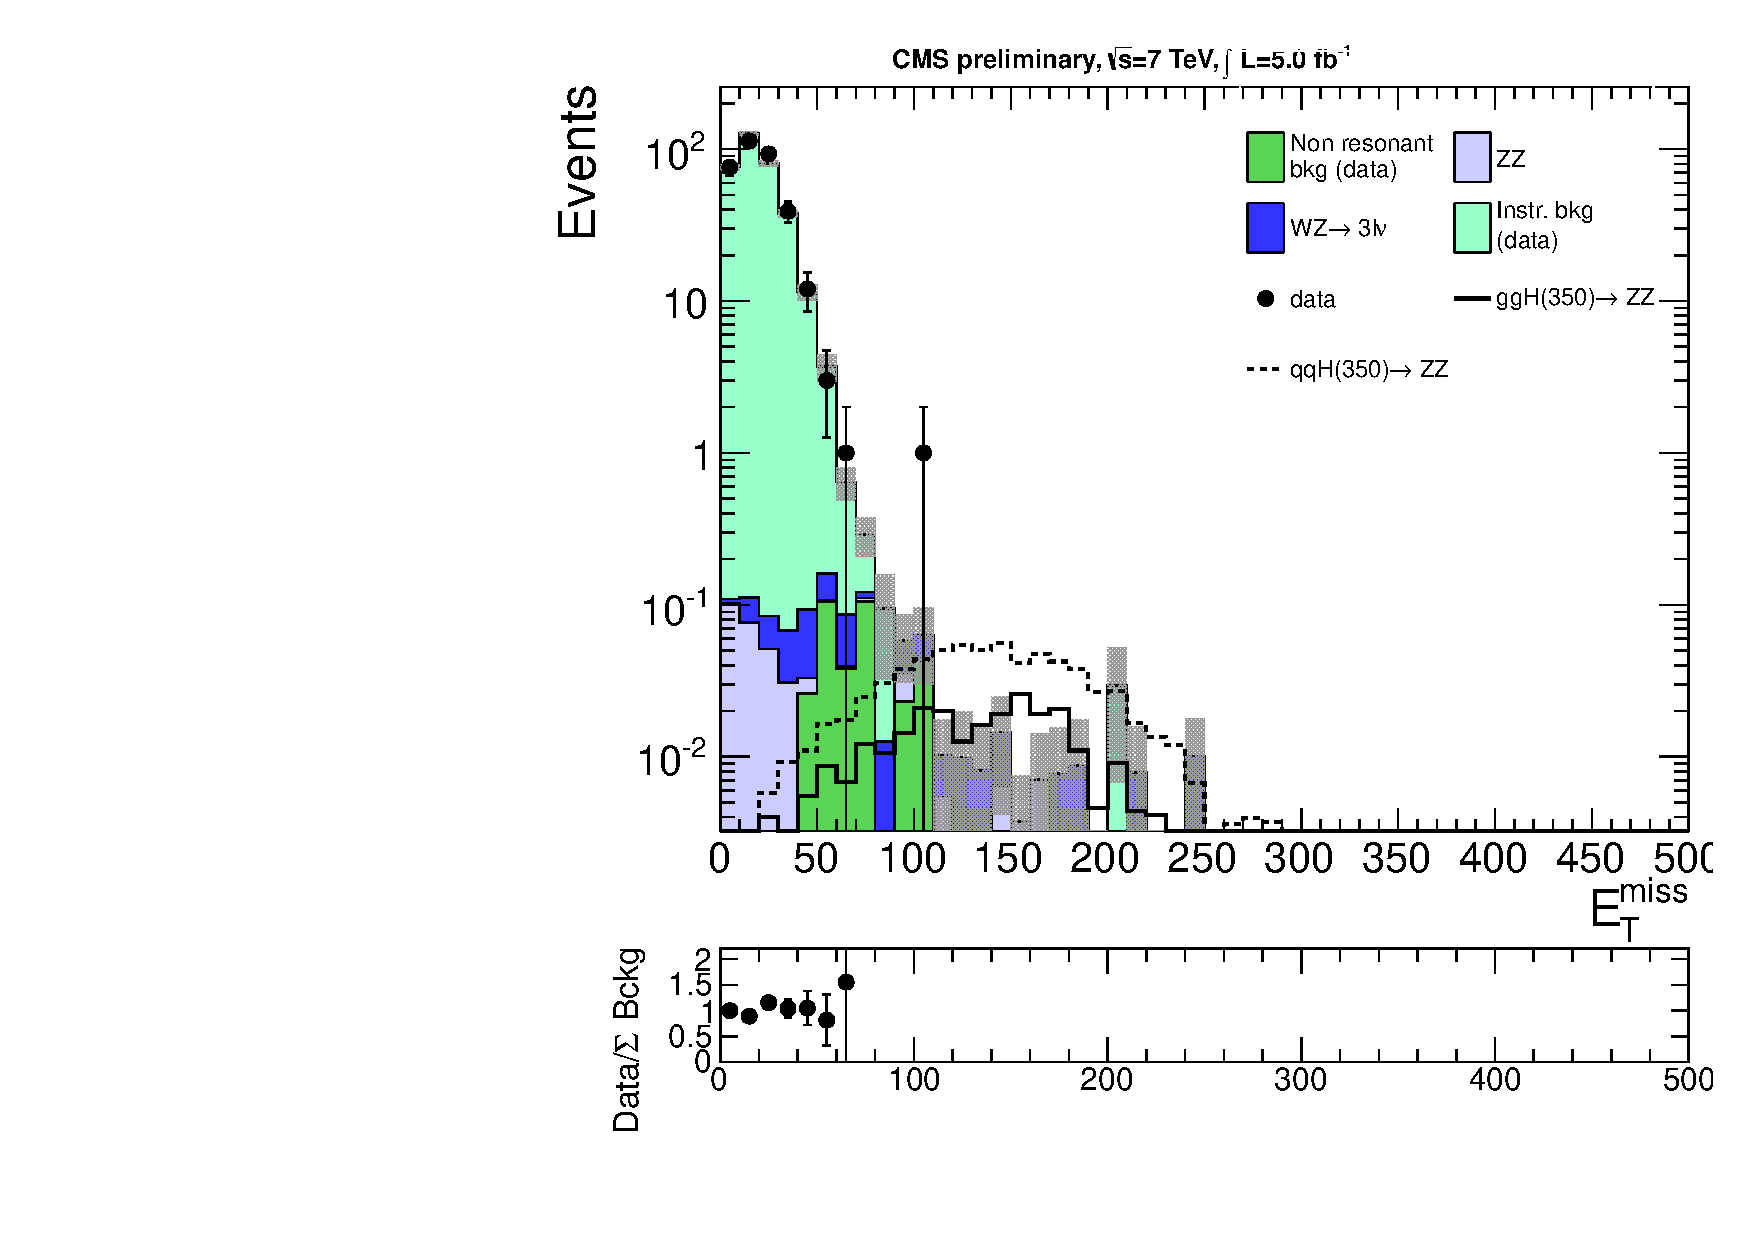
\includegraphics[width=0.48\textwidth]{plots/met_7TeV_vbf.pdf}}\\
%\subfigure[]{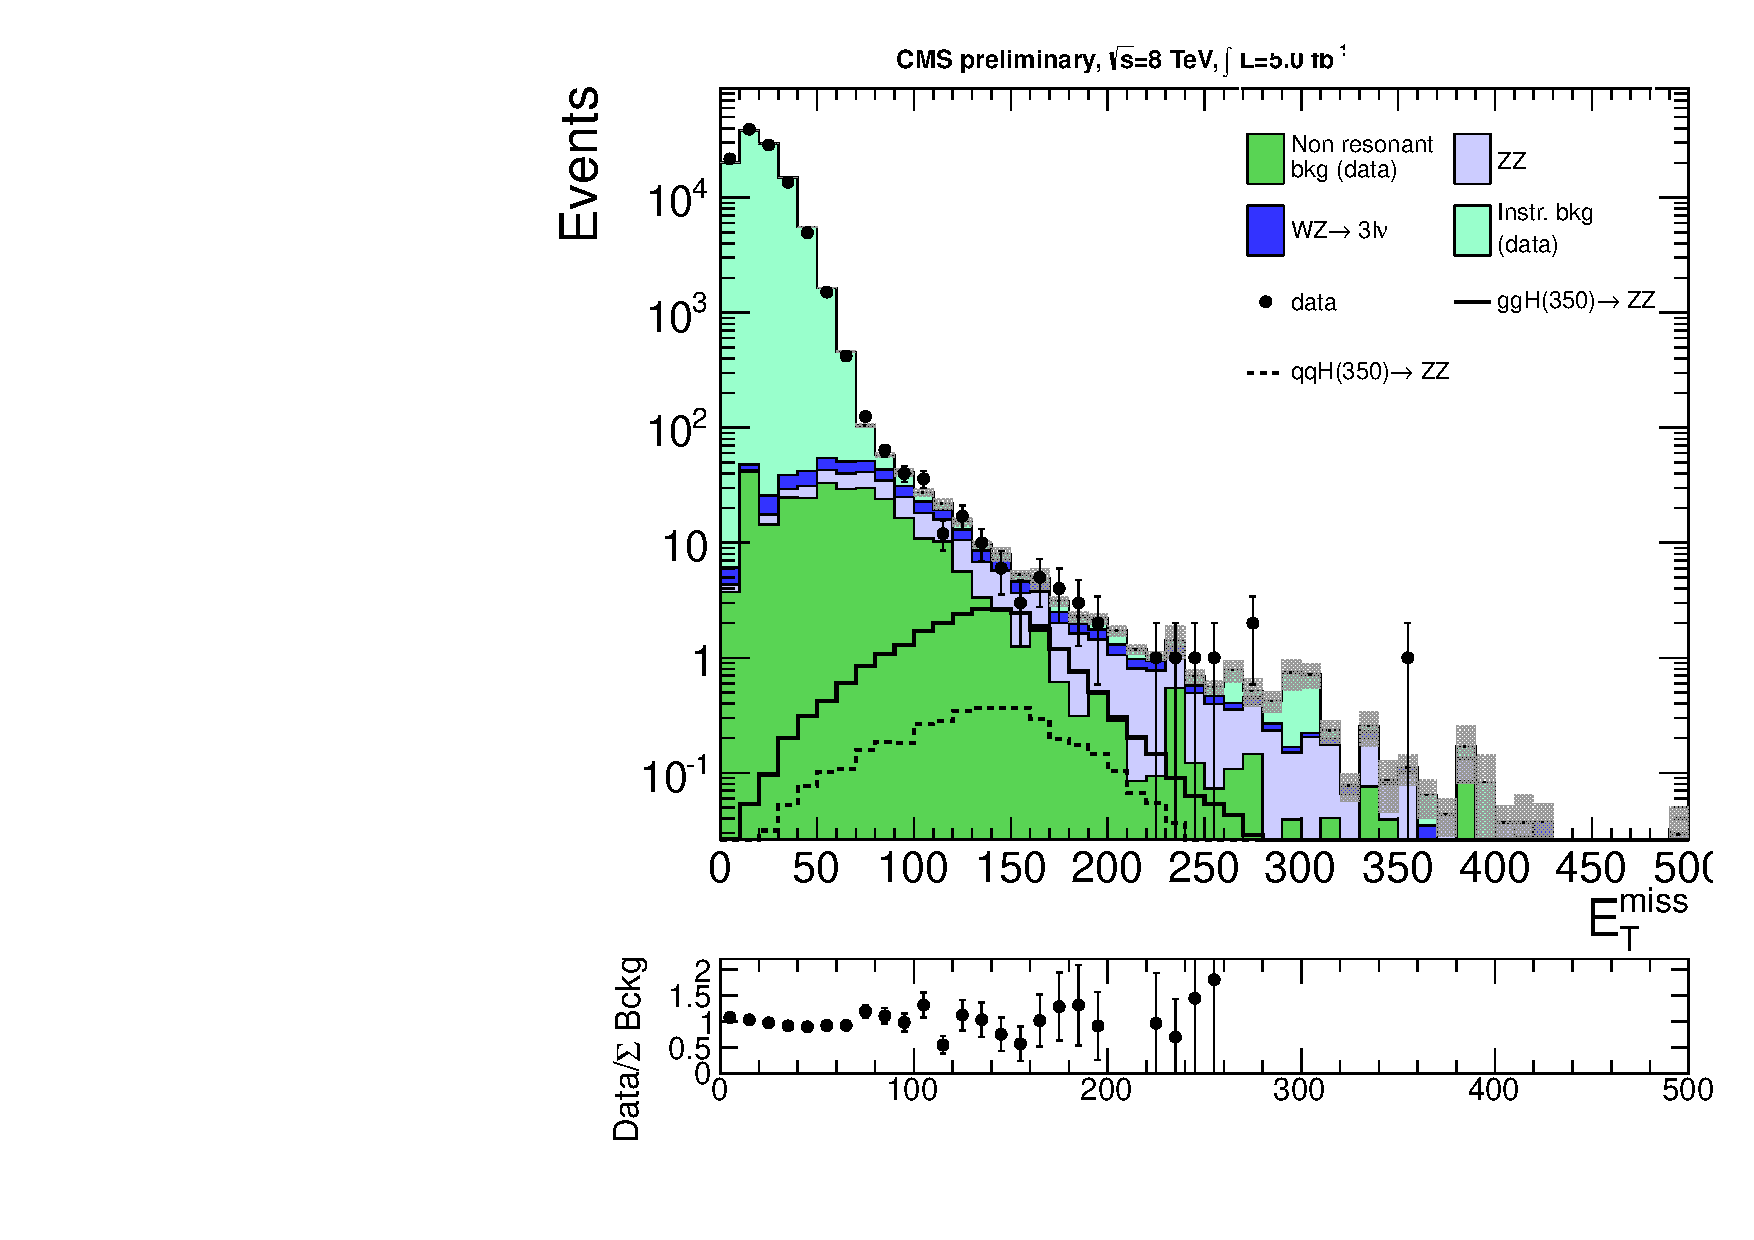
\includegraphics[width=0.48\textwidth]{plots/met_8TeV.pdf}}
%\subfigure[]{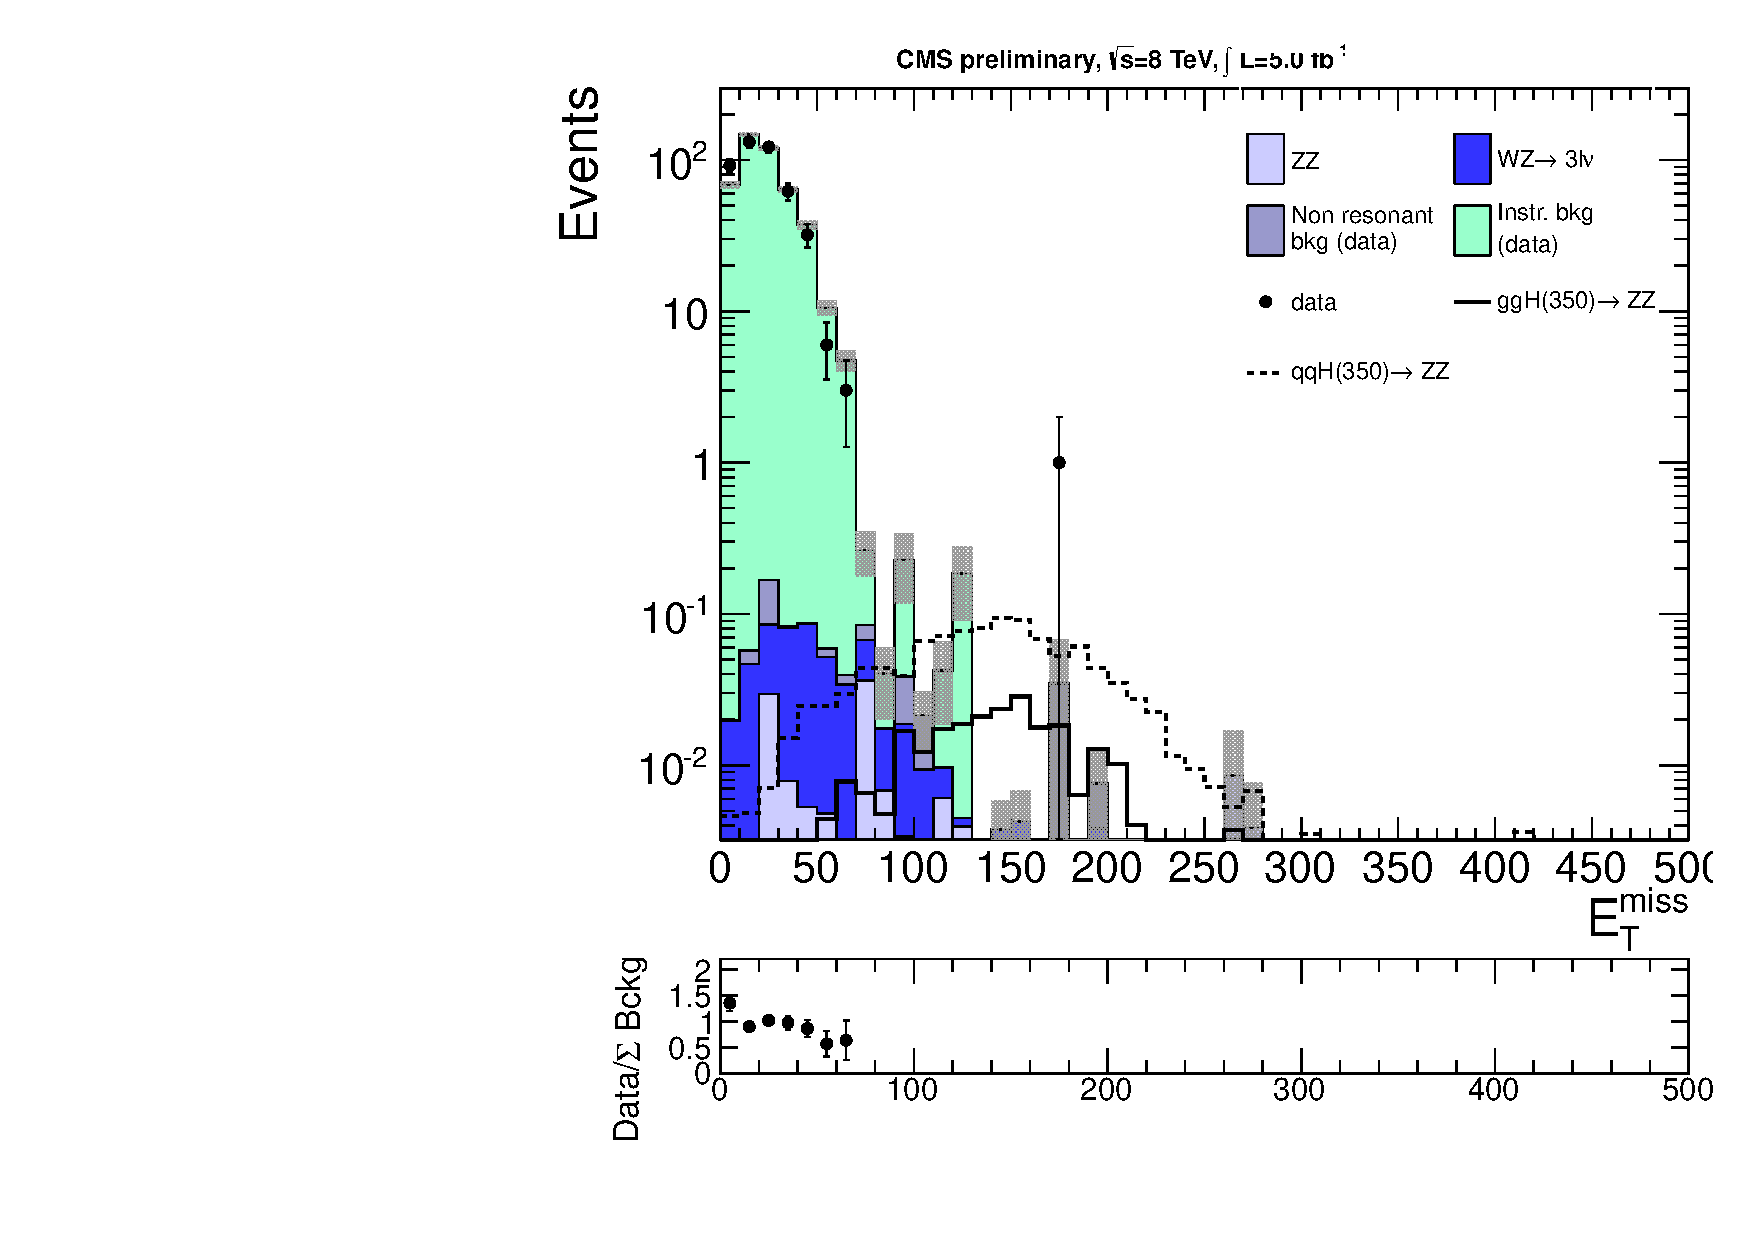
\includegraphics[width=0.48\textwidth]{plots/met_8TeV_vbf.pdf}}
\subfigure[]{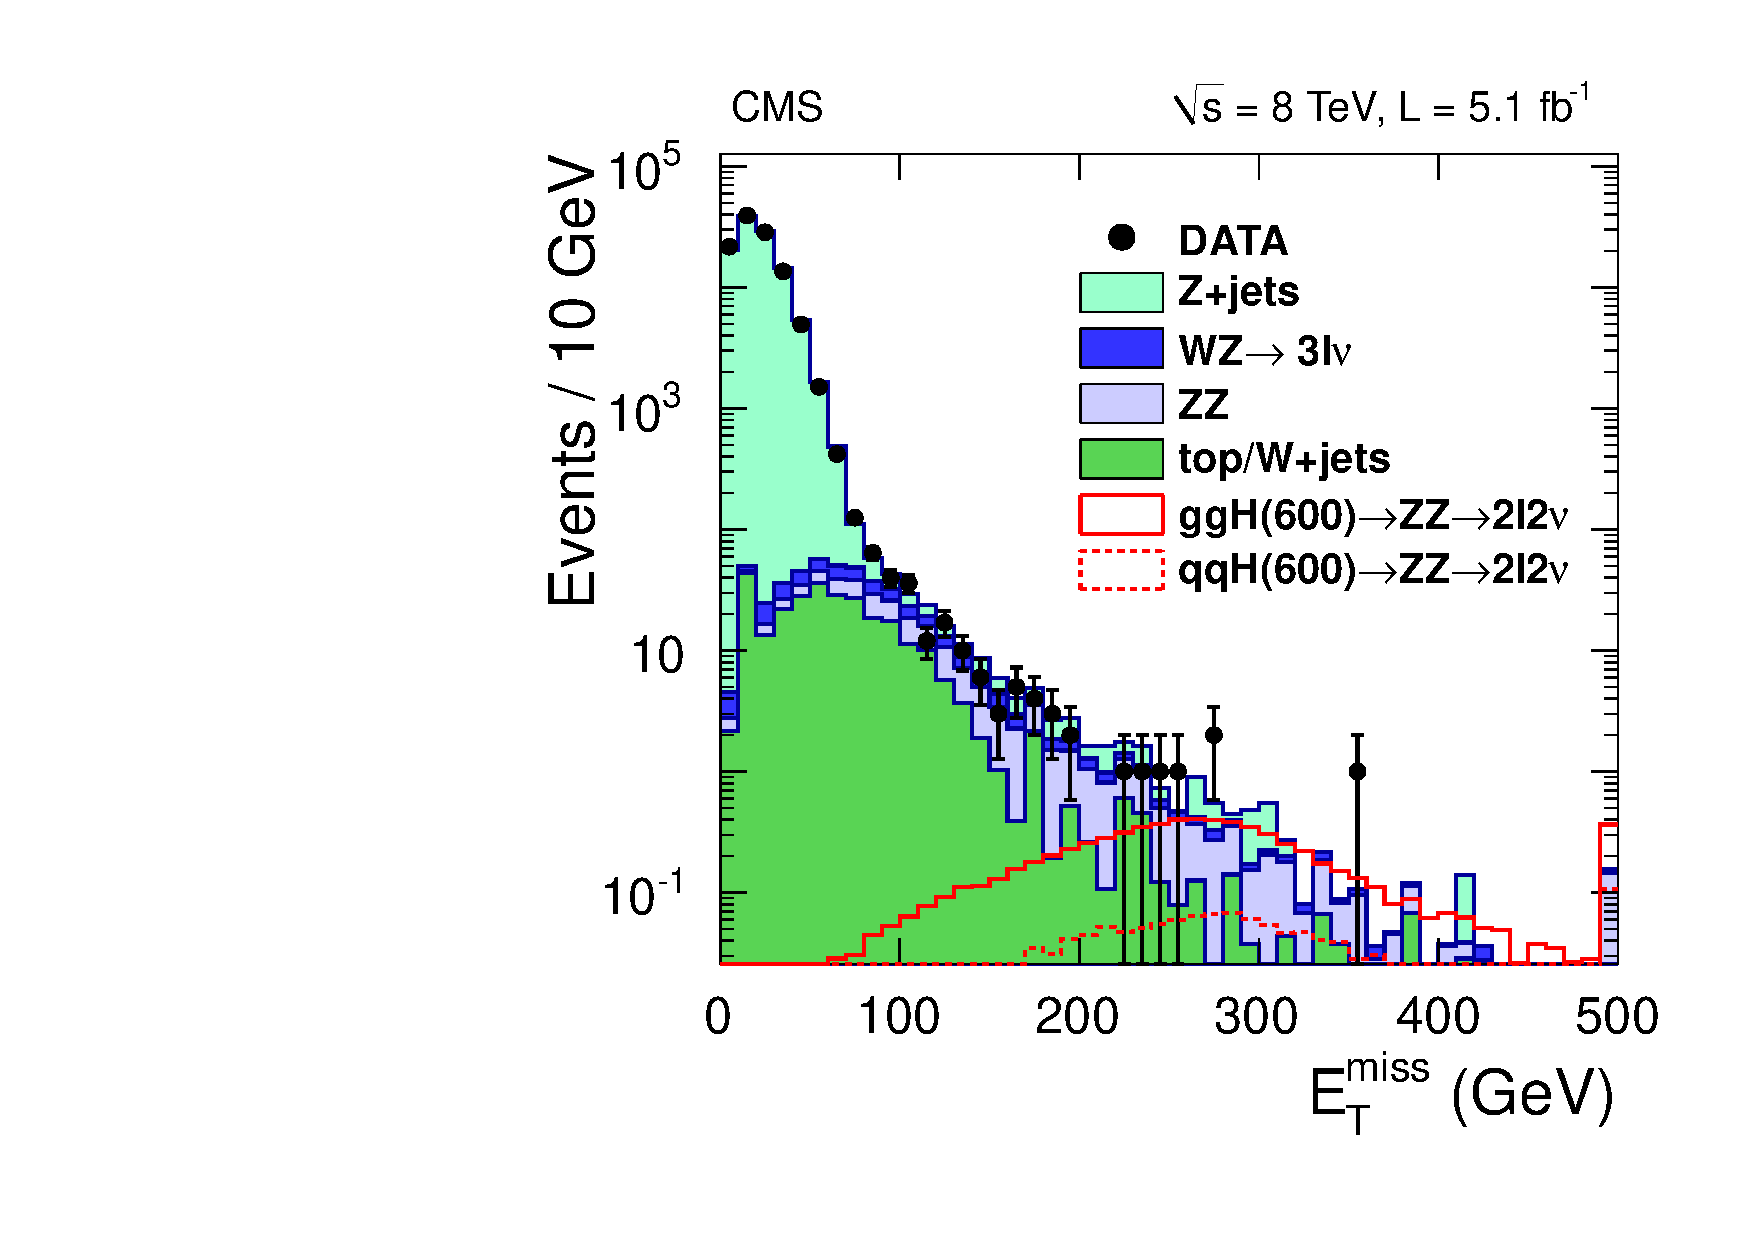
\includegraphics[width=0.45\textwidth]{figures/ZZ2l2nuNoVBF.pdf}}
\subfigure[]{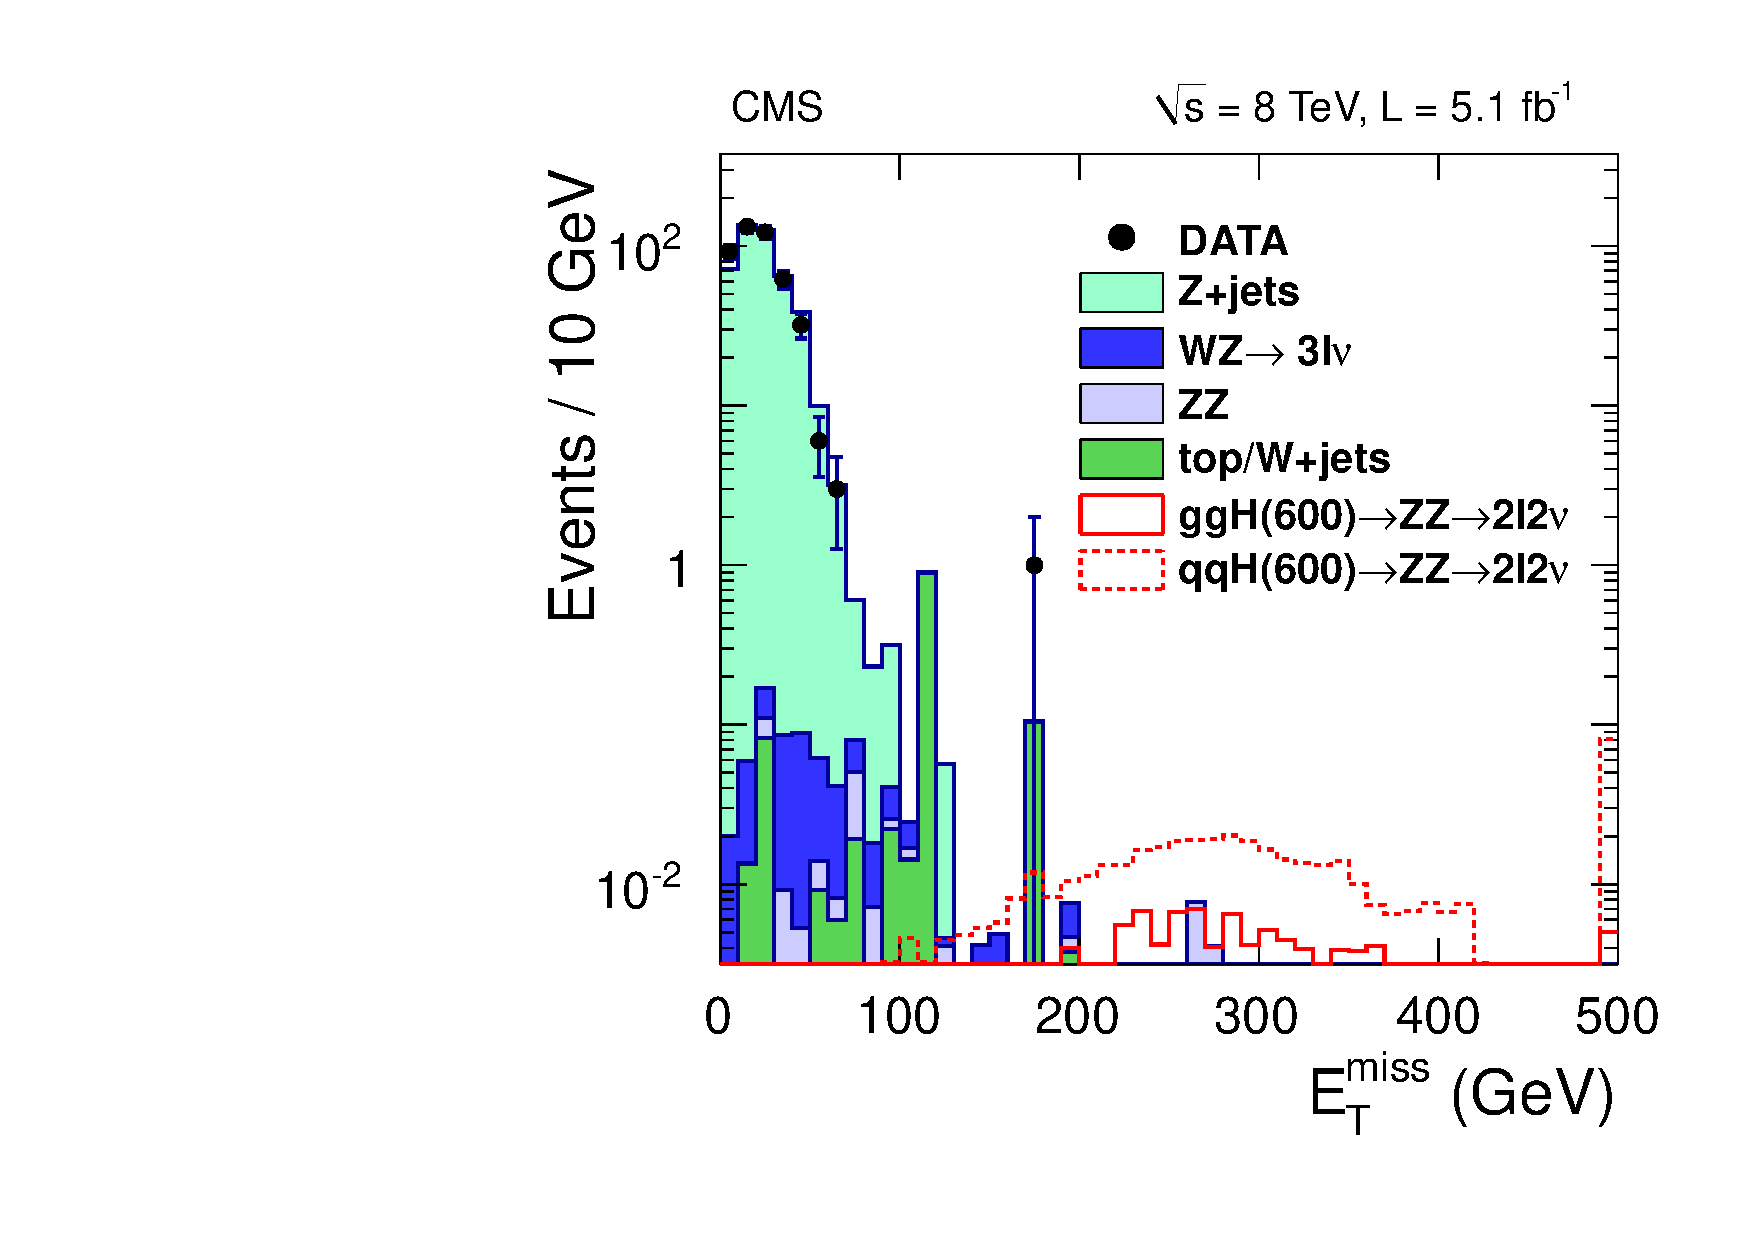
\includegraphics[width=0.45\textwidth]{figures/ZZ2l2nuVBF.pdf}}
\caption{The \MET distribution in data compared to the estimated background from data or simulation
in the (a) gluon fusion and (b) VBF categories. 
The dielectron and dimuon channels are combined.
Contributions from $\ZZ$, $\PW\cPZ$, non-resonant background and $\cPZ$+jets background are stacked
on top of each other. The \MET distribution in signal events for $\mH = 350$\GeV is also shown. The small plots below the \MET distributions show the ratio
of observed data to expected background events. Note that the scale of the y-axis is zoomed in around 1 and a few outliers appear as empty bins.}
\label{fig:zgamma_met_data}
\end{center}
\end{figure}

The uncertainty on the prediction of the $\cPZ$+jets background is affected by any
residual contamination of the $\Pgg$+jets control sample from processes involving
a photon and genuine $\MET$. We do not explicitly subtract this contamination and 
instead estimate this background conservatively to be 50\% 
of the background estimate and assign a 100\% uncertainty to it, effectively allowing the limit fit to determine the most likely amount. 

The background processes that do not involve a $\cPZ$ resonance (non-resonant background)
are estimated with a control sample of events with dileptons of different flavor
($\Pe^{\pm}\Pgm^{\mp}$) that pass the full analysis selection.
%This background consists mainly of leptonic \PW\ decays in $\ttbar$, $\cPqt\PW$ decays and
%$\PW\PW$ events. Small contributions from single top-quark events produced from
%$s$-channel and $t$-channel processes, $\PW$+jets events in which the $\PW$ boson
%decays leptonically and a jet is mismeasured as a lepton, and $\cPZ\rightarrow \Pgt\Pgt$
%events in which $\Pgt$ leptons produce light leptons and \MET are included in this estimate of the non-resonant background.
This method cannot distinguish between the non-resonant background and
a possible contribution from $\PH \rightarrow \PW\PW \rightarrow 2\ell 2\cPgn$ events, which are treated
as part of the non-resonant background estimate.
The non-resonant background in the $\Pep\Pem$ and $\Pgmp\Pgmm$ final states
is estimated by applying a scale factor to the selected
$\Pe^{\pm}\Pgm^{\mp}$ events.
%\begin{equation*}
%N_{\Pgm\Pgm} = \alpha_{\Pgm} \times N_{\Pe\Pgm}, \qquad
%N_{\Pe\Pe} = \alpha_{\Pe} \times N_{\Pe\Pgm}.
%\end{equation*}
The scale factor is computed from the sidebands of the $\cPZ$ peak events
(40 $< m_{\ell\ell} <$ 70\GeV and 110~ $< m_{\ell\ell} <$200\GeV).
% by using the following relations:
%\begin{equation*}
%\alpha_{\Pgm} = \frac{N_{\Pgm\Pgm}^\mathrm{SB}}{N_{\Pe\Pgm}^\mathrm{SB}}, \qquad
%\alpha_{\Pe} = \frac{N_{\Pe\Pe}^\mathrm{SB}}{N_{\Pe\Pgm}^{SB}},
%\end{equation*}
%where $N_{\Pe\Pe}^\mathrm{SB}$, $N_{\Pgm\Pgm}^\mathrm{SB}$, and $N_{\Pe\Pgm}^\mathrm{SB}$ are the number of events
%in the $\cPZ$ sidebands in a top-enriched sample of $\Pep\Pem$, $\Pgmp\Pgmm$, and $\Pe^{\pm}\Pgm^{\mp}$
%final states, respectively. Such samples are selected by requiring \MET$>$70\GeV and a \cPqb-tagged jet in the events, 
%but no jet-bin requirements or VBF selection 
%are applied. 
%The measured values of $\alpha$ with the corresponding statistical uncertainties
%are $\alpha_{\Pgm}= 0.61 \pm 0.04$ and $\alpha_{\Pe} = 0.34 \pm 0.03$.
The uncertainty on the estimate of the
non-resonant background is determined to be 25\%. 
%is determined by variations found in the scale factor 
%during closure tests using simulated events as well as by 
%comparing results for $\alpha$ calculated with and without applying a b-tag veto (top enriched control region). It is found to be 25\%. 
%As a cross check we estimate the EWK photon contamination from MC simulation and subtract it 
%from the data driven estimate. The resulting contribution to the limit calculation is very similar in both cases. 
%Given that the background remaining after all selection requirements is very
%small, the large uncertainty on it is of low importance.
The signal and background expected as well as observed event yields for 
$\mH=400\GeV$ hypothesis are 
listed in Table~\ref{tab:final_yields}.
No significant excess of events is observed over the expectation from the SM background.

%============
\begin{table}[htbp]
\begin{center}
\caption{
The number of event candidates observed, compared to the mean expected 
background and signal yields for each category.
}
\label{tab:final_yields}
\begin{tabular}{l|c|c|c}
\hline
Category & VBF & 0jets & $\geq$1 jets \\
\hline
Background &  3.0 $\pm$ 0.9 $\pm$ 0.4 &  13.8 $\pm$ 0.6 $\pm$ 1.4  &  20.6 $\pm$ 0.9 $\pm$ 3.1 \\ %
\hline
Observed  & 2 & 13  & 24 \\ %
\hline
$\mH = 400\GeV$ & 2.0 $\pm$ 0.1 & 17.2 $\pm$ 0.1 & 22.1 $\pm$ 0.1 \\ % 
\hline
\end{tabular}
\end{center}
\end{table}

The observed and expected 
upper limits 
%cross section $\sigma$ to the SM Higgs boson production cross section
%$\sigma_\mathrm{SM}$ 
as a function of $\mH$ are shown in Fig.~\ref{fig:limits_SM}.
% for 7\TeV and 8\TeV separately and for both years
%combined.
The SM Higgs boson is excluded
in the mass range 220--675\GeV at 95\% confidence level, while the
expected exclusion limit in the background-only hypothesis is 275--630\GeV.

\begin{figure}[htbp]
\begin{center}
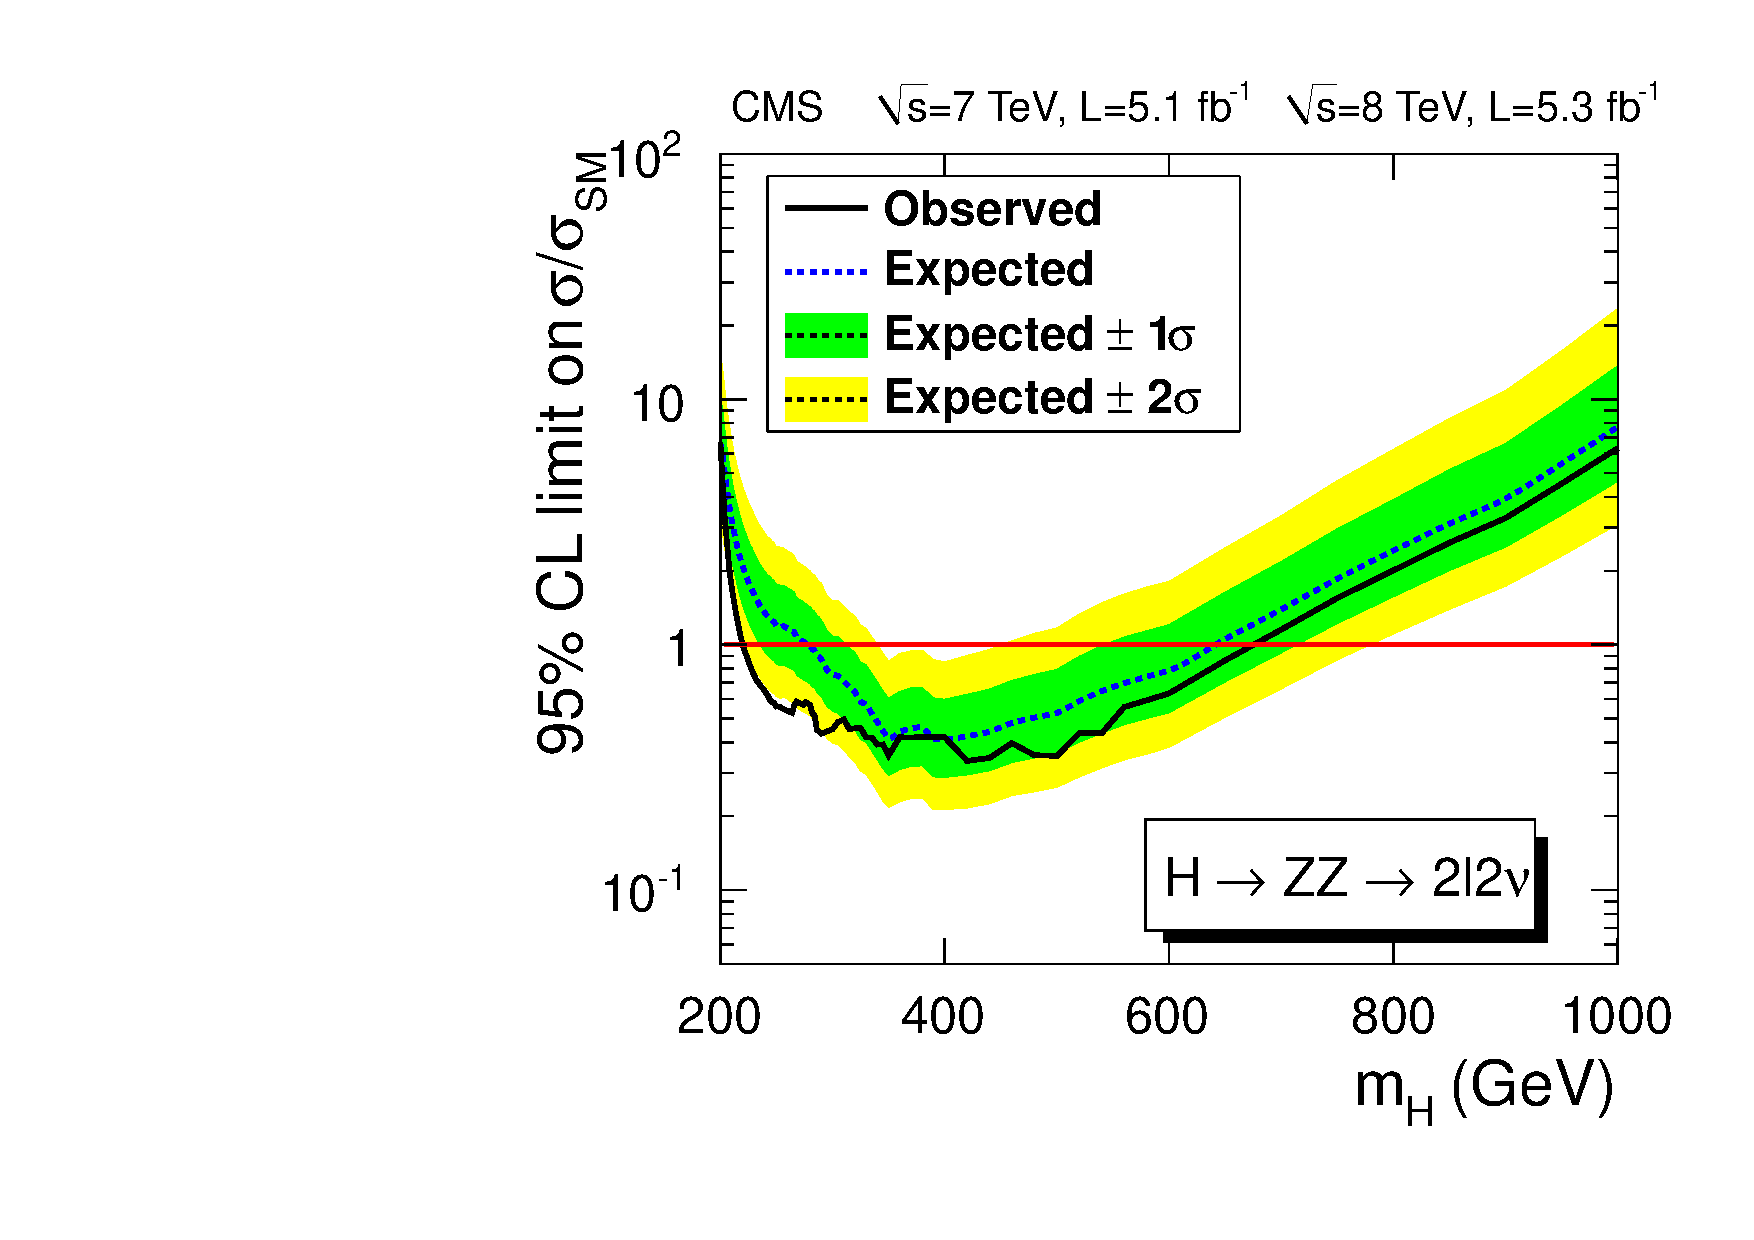
\includegraphics[width=0.6\textwidth]{figures/ZZ2l2nuLimit.pdf}
\caption{Observed (solid) and expected
(dashed) 95\% CL upper limit on the ratio of the production cross
section to the SM expectation for the Higgs boson.
} 
\label{fig:limits_SM}
\end{center}
\end{figure}
